% \documentclass[a4paper,10pt]{article} % or whatever
% \documentclass[letterpaper,10pt]{article} % or whatever
\documentclass{article}

% if you need to pass options to natbib, use, e.g.:
     \PassOptionsToPackage{numbers, compress}{natbib}

\usepackage[preprint]{neurips_2021}

\newcommand{\ignore}[1]{}
% to avoid loading the natbib package, add option nonatbib:
\usepackage{dsfont}

% Note: this has been tested using MiKTeX 2.9. If you are getting errors, update your packages.

%%% Packages %%%
%\usepackage{setspace} % Double spaces document. Footnotes,
                      % figures, and tables will still be single spaced, however.
%\doublespacing
%\singlespacing
%\onehalfspacing
% \setstretch{1.5} % set double spacing to 1.5 or anything else.

\usepackage[T1]{fontenc}
\usepackage{amsmath,amssymb,amsfonts,mathrsfs,bm}% Typical maths resource packages
\usepackage{mathtools}
%\let\proof\relax
%\let\endproof\relax
\usepackage{amsthm}
\usepackage{nicefrac}
%\usepackage{cite}
%\let\labelindent\relax
\usepackage[shortlabels]{enumitem}
\usepackage{graphicx}
\usepackage{epstopdf}
\usepackage{url}
\usepackage{colortbl}
\usepackage{booktabs}
\usepackage{multirow}
\usepackage[table,dvipsnames]{xcolor}
\usepackage[normalem]{ulem}
\usepackage{xparse}

%\usepackage{pstricks}
%\usepackage{psfrag}
%\usepackage{syntonly}
%\syntaxonly
%\usepackage[style=base]{caption}
%\captionsetup{
    %format = plain,
    %font = footnotesize,
    %labelfont = sc
%}


\usepackage{array}
\newcolumntype{L}[1]{>{\raggedright\let\newline\\\arraybackslash\hspace{0pt}}m{#1}}
\newcolumntype{C}[1]{>{\centering\let\newline\\\arraybackslash\hspace{0pt}}m{#1}}
\newcolumntype{R}[1]{>{\raggedleft\let\newline\\\arraybackslash\hspace{0pt}}m{#1}}

\makeatletter
\let\MYcaption\@makecaption
\makeatother
\usepackage[font=footnotesize]{subcaption}
\makeatletter
\let\@makecaption\MYcaption
\makeatother


% achieves the functionality of \tag for subequations environment
\makeatletter
\newenvironment{varsubequations}[1]
 {%
  \addtocounter{equation}{-1}%
  \begin{subequations}
  \renewcommand{\theparentequation}{#1}%
  \def\@currentlabel{#1}%
 }
 {%
  \end{subequations}\ignorespacesafterend
 }
\makeatother


\usepackage{glossaries}

\makeatletter
% copy old \gls and \glspl
\let\oldgls\gls
\let\oldglspl\glspl

% define a non space skipping version of \@ifnextchar
\newcommand\fussy@ifnextchar[3]{%
  \let\reserved@d=#1%
  \def\reserved@a{#2}%
  \def\reserved@b{#3}%
  \futurelet\@let@token\fussy@ifnch}
\def\fussy@ifnch{%
  \ifx\@let@token\reserved@d
    \let\reserved@c\reserved@a 
  \else
    \let\reserved@c\reserved@b
  \fi
 \reserved@c}

\renewcommand{\gls}[1]{%
  \oldgls{#1}\fussy@ifnextchar.{\@checkperiod}{\@}}
\renewcommand{\glspl}[1]{%
  \oldglspl{#1}\fussy@ifnextchar.{\@checkperiod}{\@}}

\newcommand{\@checkperiod}[1]{%
  \ifnum\sfcode`\.=\spacefactor\else#1\fi
}
\makeatother

%%%%%%%%%%%%% new add %%%%%%%%%%%%% 
\newcommand{\tb}[1]{\textbf{#1}}


\newacronym{wrt}{w.r.t.}{with respect to}
\newacronym{RHS}{R.H.S.}{right-hand side}
\newacronym{LHS}{L.H.S.}{left-hand side}
\newacronym{iid}{i.i.d.}{independent and identically distributed}
%\newacronym{MIMO}{MIMO}{mulitple-input multiple-output}
%\newacronym{AOA}{AOA}{angle-of-arrival}
%\newacronym{AOD}{AOD}{angle-of-departure}
%\newacronym{LOS}{LOS}{line-of-sight}
%\newacronym{NLOS}{NLOS}{non-line-of-sight}
%\newacronym{TOA}{TOA}{time-of-arrival}
%\newacronym{TDOA}{TDOA}{time-difference-of-arrival}
%\newacronym{RSS}{RSS}{received signal strength}
%\newacronym{GNSS}{GNSS}{Global Navigation Satellite System}
%\newacronym{GSP}{GSP}{graph signal processing}
%\newacronym{ML}{ML}{machine learning}


%put the float package before hyperref and algorithm package after hyperref for hyperref to work correctly with algorithm
\usepackage{float}

\ifx\notloadhyperref\undefined
	\ifx\loadbibentry\undefined
		\usepackage[hidelinks,hypertexnames=false]{hyperref} 
	\else
		\usepackage{bibentry}
		\makeatletter\let\saved@bibitem\@bibitem\makeatother
		\usepackage[hidelinks,hypertexnames=false]{hyperref}
		\makeatletter\let\@bibitem\saved@bibitem\makeatother
	\fi
\else
	\ifx\loadbibentry\undefined
		\relax
	\else
		\usepackage{bibentry}
	\fi
\fi

\usepackage[capitalize]{cleveref}
\crefname{equation}{}{}
\Crefname{equation}{}{}
\crefname{claim}{claim}{claims}
\crefname{step}{step}{steps}
\crefname{line}{line}{lines}
\crefname{condition}{condition}{conditions}
\crefname{dmath}{}{}
\crefname{dseries}{}{}
\crefname{dgroup}{}{}

\crefname{Problem}{Problem}{Problems}
\crefformat{Problem}{Problem~(#2#1#3)}
\crefrangeformat{Problem}{Problems~(#3#1#4) to~(#5#2#6)}

\crefname{Theorem}{Theorem}{Theorems}
\crefname{Corollary}{Corollary}{Corollaries}
\crefname{Proposition}{Proposition}{Propositions}
\crefname{Lemma}{Lemma}{Lemmas}
\crefname{Definition}{Definition}{Definitions}
\crefname{Example}{Example}{Examples}
\crefname{Assumption}{Assumption}{Assumptions}
\crefname{Remark}{Remark}{Remarks}
\crefname{Rem}{Remark}{Remarks}
\crefname{remarks}{Remarks}{Remarks}
\crefname{Appendix}{Appendix}{Appendices}
\crefname{Supplement}{Supplement}{Supplements}
\crefname{Exercise}{Exercise}{Exercises}
\crefname{Theorem_A}{Theorem}{Theorems}
\crefname{Corollary_A}{Corollary}{Corollaries}
\crefname{Proposition_A}{Proposition}{Propositions}
\crefname{Lemma_A}{Lemma}{Lemmas}
\crefname{Definition_A}{Definition}{Definitions}
\crefname{rema}{Remark}{Remarks}
\crefname{exma}{Example}{Examples}

\usepackage{crossreftools}
\ifx\notloadhyperref\undefined
	\pdfstringdefDisableCommands{%
			\let\Cref\crtCref
			\let\cref\crtcref
	}
\else
	\relax
\fi

\usepackage{algorithm,algorithmic}
\renewcommand{\algorithmicrequire}{\textbf{Input:}}
\renewcommand{\algorithmicensure}{\textbf{Output:}}

%may cause conflict with some packages like tikz, include manually if desired
%load after hyperref
\ifx\loadbreqn\undefined
	\relax
\else
	\usepackage{breqn} 
\fi



%%%%%%%%%%%%%%%%%%%%%%%%%%%%%%%%%%%%%%%%%%%%%%%%


\interdisplaylinepenalty=2500   % To restore IEEEtran ability to automatically break
                                % within multiline equations, when using amsmath.

%%%%%%%%%%%%%%%%%%%%%%%%%%%%%%%%%%%%%%%%

%Theorem declarations

\ifx\renewtheorem\undefined
% for use in main body
\ifx\useTheoremCounter\undefined
\newtheorem{Theorem}{Theorem}
\newtheorem{Corollary}{Corollary}
\newtheorem{Proposition}{Proposition}
\newtheorem{Lemma}{Lemma}
\else
\newtheorem{Theorem}{Theorem}
\newtheorem{Corollary}[theorem]{Corollary}
\newtheorem{Proposition}[theorem]{Proposition}
\fi

\newtheorem{Definition}{Definition}
\newtheorem{Example}{Example}
\newtheorem{Remark}{Remark}
\newtheorem{Assumption}{Assumption}
\newtheorem{Exercise}{Exercise}

% for use in the appendix
\newtheorem{Theorem_A}{Theorem}[section]
\newtheorem{Corollary_A}{Corollary}[section]
\newtheorem{Proposition_A}{Proposition}[section]
\newtheorem{Lemma_A}{Lemma}[section]
\newtheorem{Definition_A}{Definition}[section]
\fi

\usepackage{amsmath}
\numberwithin{equation}{section} % or whatever you prefer
% \swapnumbers % I prefer this
% \theoremstyle{plain}
\newtheorem{thma}[equation]{Theorem}
\newtheorem{propa}[equation]{Proposition}
\newtheorem{lema}[equation]{Lemma}
\newtheorem{defa}[equation]{Definition}
\newtheorem{cora}[equation]{Corollary}
\newtheorem{Lemma_AA}{Lemma}[section]
\newtheorem{rema}[equation]{Remark}
\newtheorem{exma}[equation]{Example}
\newcommand{\ml}[1]{\begin{multlined}#1\end{multlined}}
\newcommand{\nn}{\nonumber\\ }


% Remarks
\theoremstyle{remark}
\newtheorem{Rem}{Remark}
\theoremstyle{plain}

\newenvironment{remarks}{
	\begin{list}{\textit{Remark} \arabic{Rem}:~}{
    \setcounter{enumi}{\value{Rem}}
    \usecounter{Rem}
    \setcounter{Rem}{\value{enumi}}
    \setlength\labelwidth{0in}
    \setlength\labelsep{0in}
    \setlength\leftmargin{0in}
    \setlength\listparindent{0in}
    \setlength\itemindent{15pt}
		}
}{
	\end{list}
}


% Special Headings
%\newtheorem*{Prop1}{Proposition 1} %needs amsthm

%\newtheoremstyle{nonum}{}{}{\itshape}{}{\bfseries}{.}{ }{#1 (\mdseries #3)}
%\theoremstyle{nonum}
%\newtheorem{Example**}{Example 1}

\newcommand{\EndExample}{{$\square$}}
%\renewcommand{\QED}{\QEDopen} % changes end of proof box to open box.

\newcommand{\qednew}{\nobreak \ifvmode \relax \else
      \ifdim\lastskip<1.5em \hskip-\lastskip
      \hskip1.5em plus0em minus0.5em \fi \nobreak
      \vrule height0.75em width0.5em depth0.25em\fi}


%\newcommand{\em}[1]{\emph{#1}}

% Move down subscripts for some symbols like \chi
\NewDocumentCommand{\movedownsub}{e{^_}}{%
  \IfNoValueTF{#1}{%
    \IfNoValueF{#2}{^{}}% neither ^ nor _, do nothing; if no ^ but _, add ^{}
  }{%
    ^{#1}% add superscript if present
  }%
  \IfNoValueF{#2}{_{#2}}% add subscript if present
}



%Number sets
\newcommand{\Real}{\mathbb{R}}
\newcommand{\Nat}{\mathbb{N}}
\newcommand{\Rat}{\mathbb{Q}}
\newcommand{\Complex}{\mathbb{C}}

% imaginary number i
\newcommand{\iu}{\mathfrak{i}\mkern1mu}


% Calligraphic stuff
\newcommand{\calA}{\mathcal{A}}
\newcommand{\calB}{\mathcal{B}}
\newcommand{\calC}{\mathcal{C}}
\newcommand{\calD}{\mathcal{D}}
\newcommand{\calE}{\mathcal{E}}
\newcommand{\calF}{\mathcal{F}}
\newcommand{\calG}{\mathcal{G}}
\newcommand{\calH}{\mathcal{H}}
\newcommand{\calI}{\mathcal{I}}
\newcommand{\calJ}{\mathcal{J}}
\newcommand{\calK}{\mathcal{K}}
\newcommand{\calL}{\mathcal{L}}
\newcommand{\calM}{\mathcal{M}}
\newcommand{\calN}{\mathcal{N}}
\newcommand{\calO}{\mathcal{O}}
\newcommand{\calP}{\mathcal{P}}
\newcommand{\calQ}{\mathcal{Q}}
\newcommand{\calR}{\mathcal{R}}
\newcommand{\calS}{\mathcal{S}}
\newcommand{\calT}{\mathcal{T}}
\newcommand{\calU}{\mathcal{U}}
\newcommand{\calV}{\mathcal{V}}
\newcommand{\calW}{\mathcal{W}}
\newcommand{\calX}{\mathcal{X}}
\newcommand{\calY}{\mathcal{Y}}
\newcommand{\calZ}{\mathcal{Z}}

% Boldface stuff
\newcommand{\ba}{\mathbf{a}}
\newcommand{\bA}{\mathbf{A}}
\newcommand{\bb}{\mathbf{b}}
\newcommand{\bB}{\mathbf{B}}
\newcommand{\bc}{\mathbf{c}}
\newcommand{\bC}{\mathbf{C}}
\newcommand{\bd}{\mathbf{d}}
\newcommand{\bD}{\mathbf{D}}
\newcommand{\be}{\mathbf{e}}
\newcommand{\bE}{\mathbf{E}}
\newcommand{\boldf}{\mathbf{f}}
\newcommand{\bF}{\mathbf{F}}
\newcommand{\bg}{\mathbf{g}}
\newcommand{\bG}{\mathbf{G}}
\newcommand{\bh}{\mathbf{h}}
\newcommand{\bH}{\mathbf{H}}
\newcommand{\bi}{\mathbf{i}}
\newcommand{\bI}{\mathbf{I}}
\newcommand{\bj}{\mathbf{j}}
\newcommand{\bJ}{\mathbf{J}}
\newcommand{\bk}{\mathbf{k}}
\newcommand{\bK}{\mathbf{K}}
\newcommand{\bl}{\mathbf{l}}
\newcommand{\bL}{\mathbf{L}}
\newcommand{\boldm}{\mathbf{m}}
\newcommand{\bM}{\mathbf{M}}
\newcommand{\bn}{\mathbf{n}}
\newcommand{\bN}{\mathbf{N}}
\newcommand{\bo}{\mathbf{o}}
\newcommand{\bO}{\mathbf{O}}
\newcommand{\bp}{\mathbf{p}}
\newcommand{\bP}{\mathbf{P}}
\newcommand{\bq}{\mathbf{q}}
\newcommand{\bQ}{\mathbf{Q}}
\newcommand{\br}{\mathbf{r}}
\newcommand{\bR}{\mathbf{R}}
\newcommand{\bs}{\mathbf{s}}
\newcommand{\bS}{\mathbf{S}}
\newcommand{\bt}{\mathbf{t}}
\newcommand{\bT}{\mathbf{T}}
\newcommand{\bu}{\mathbf{u}}
\newcommand{\bU}{\mathbf{U}}
\newcommand{\bv}{\mathbf{v}}
\newcommand{\bV}{\mathbf{V}}
\newcommand{\bw}{\mathbf{w}}
\newcommand{\bW}{\mathbf{W}}
\newcommand{\bx}{\mathbf{x}}
\newcommand{\bX}{\mathbf{X}}
\newcommand{\by}{\mathbf{y}}
\newcommand{\bY}{\mathbf{Y}}
\newcommand{\bz}{\mathbf{z}}
\newcommand{\bZ}{\mathbf{Z}}


\newcommand{\mba}{\bm{a}}
\newcommand{\mbA}{\bm{A}}
\newcommand{\mbb}{\bm{b}}
\newcommand{\mbB}{\bm{B}}
\newcommand{\mbc}{\bm{c}}
\newcommand{\mbC}{\bm{C}}
\newcommand{\mbd}{\bm{d}}
\newcommand{\mbD}{\bm{D}}
\newcommand{\mbe}{\bm{e}}
\newcommand{\mbE}{\bm{E}}
\newcommand{\mbf}{\bm{f}}
\newcommand{\mbF}{\bm{F}}
\newcommand{\mbg}{\bm{g}}
\newcommand{\mbG}{\bm{G}}
\newcommand{\mbh}{\bm{h}}
\newcommand{\mbH}{\bm{H}}
\newcommand{\mbi}{\bm{i}}
\newcommand{\mbI}{\bm{I}}
\newcommand{\mbj}{\bm{j}}
\newcommand{\mbJ}{\bm{J}}
\newcommand{\mbk}{\bm{k}}
\newcommand{\mbK}{\bm{K}}
\newcommand{\mbl}{\bm{l}}
\newcommand{\mbL}{\bm{L}}
\newcommand{\mbm}{\bm{m}}
\newcommand{\mbM}{\bm{M}}
\newcommand{\mbn}{\bm{n}}
\newcommand{\mbN}{\bm{N}}
\newcommand{\mbo}{\bm{o}}
\newcommand{\mbO}{\bm{O}}
\newcommand{\mbp}{\bm{p}}
\newcommand{\mbP}{\bm{P}}
\newcommand{\mbq}{\bm{q}}
\newcommand{\mbQ}{\bm{Q}}
\newcommand{\mbr}{\bm{r}}
\newcommand{\mbR}{\bm{R}}
\newcommand{\mbs}{\bm{s}}
\newcommand{\mbS}{\bm{S}}
\newcommand{\mbt}{\bm{t}}
\newcommand{\mbT}{\bm{T}}
\newcommand{\mbu}{\bm{u}}
\newcommand{\mbU}{\bm{U}}
\newcommand{\mbv}{\bm{v}}
\newcommand{\mbV}{\bm{V}}
\newcommand{\mbw}{\bm{w}}
\newcommand{\mbW}{\bm{W}}
\newcommand{\mbx}{\bm{x}}
\newcommand{\mbX}{\bm{X}}
\newcommand{\mby}{\bm{y}}
\newcommand{\mbY}{\bm{Y}}
\newcommand{\mbz}{\bm{z}}
\newcommand{\mbZ}{\bm{Z}}

% Numbers bb font
\newcommand{\bbA}{\mathbb{A}}
\newcommand{\bbB}{\mathbb{B}}
\newcommand{\bbC}{\mathbb{C}}
\newcommand{\bbD}{\mathbb{D}}
\newcommand{\bbE}{\mathbb{E}}
\newcommand{\bbF}{\mathbb{F}}
\newcommand{\bbG}{\mathbb{G}}
\newcommand{\bbH}{\mathbb{H}}
\newcommand{\bbI}{\mathbb{I}}
\newcommand{\bbJ}{\mathbb{J}}
\newcommand{\bbK}{\mathbb{K}}
\newcommand{\bbL}{\mathbb{L}}
\newcommand{\bbM}{\mathbb{M}}
\newcommand{\bbN}{\mathbb{N}}
\newcommand{\bbO}{\mathbb{O}}
\newcommand{\bbP}{\mathbb{P}}
\newcommand{\bbQ}{\mathbb{Q}}
\newcommand{\bbR}{\mathbb{R}}
\newcommand{\bbS}{\mathbb{S}}
\newcommand{\bbT}{\mathbb{T}}
\newcommand{\bbU}{\mathbb{U}}
\newcommand{\bbV}{\mathbb{V}}
\newcommand{\bbW}{\mathbb{W}}
\newcommand{\bbX}{\mathbb{X}}
\newcommand{\bbY}{\mathbb{Y}}
\newcommand{\bbZ}{\mathbb{Z}}

% Mathfrak font
\newcommand{\frakA}{\mathfrak{A}}
\newcommand{\frakB}{\mathfrak{B}}
\newcommand{\frakC}{\mathfrak{C}}
\newcommand{\frakD}{\mathfrak{D}}
\newcommand{\frakE}{\mathfrak{E}}
\newcommand{\frakF}{\mathfrak{F}}
\newcommand{\frakG}{\mathfrak{G}}
\newcommand{\frakH}{\mathfrak{H}}
\newcommand{\frakI}{\mathfrak{I}}
\newcommand{\frakJ}{\mathfrak{J}}
\newcommand{\frakK}{\mathfrak{K}}
\newcommand{\frakL}{\mathfrak{L}}
\newcommand{\frakM}{\mathfrak{M}}
\newcommand{\frakN}{\mathfrak{N}}
\newcommand{\frakO}{\mathfrak{O}}
\newcommand{\frakP}{\mathfrak{P}}
\newcommand{\frakQ}{\mathfrak{Q}}
\newcommand{\frakR}{\mathfrak{R}}
\newcommand{\frakS}{\mathfrak{S}}
\newcommand{\frakT}{\mathfrak{T}}
\newcommand{\frakU}{\mathfrak{U}}
\newcommand{\frakV}{\mathfrak{V}}
\newcommand{\frakW}{\mathfrak{W}}
\newcommand{\frakX}{\mathfrak{X}}
\newcommand{\frakY}{\mathfrak{Y}}
\newcommand{\frakZ}{\mathfrak{Z}}

% Mathscr
\newcommand{\scA}{\mathscr{A}}
\newcommand{\scB}{\mathscr{B}}
\newcommand{\scC}{\mathscr{C}}
\newcommand{\scD}{\mathscr{D}}
\newcommand{\scE}{\mathscr{E}}
\newcommand{\scF}{\mathscr{F}}
\newcommand{\scG}{\mathscr{G}}
\newcommand{\scH}{\mathscr{H}}
\newcommand{\scI}{\mathscr{I}}
\newcommand{\scJ}{\mathscr{J}}
\newcommand{\scK}{\mathscr{K}}
\newcommand{\scL}{\mathscr{L}}
\newcommand{\scM}{\mathscr{M}}
\newcommand{\scN}{\mathscr{N}}
\newcommand{\scO}{\mathscr{O}}
\newcommand{\scP}{\mathscr{P}}
\newcommand{\scQ}{\mathscr{Q}}
\newcommand{\scR}{\mathscr{R}}
\newcommand{\scS}{\mathscr{S}}
\newcommand{\scT}{\mathscr{T}}
\newcommand{\scU}{\mathscr{U}}
\newcommand{\scV}{\mathscr{V}}
\newcommand{\scW}{\mathscr{W}}
\newcommand{\scX}{\mathscr{X}}
\newcommand{\scY}{\mathscr{Y}}
\newcommand{\scZ}{\mathscr{Z}}


% define some useful uppercase Greek letters in regular and bold sf
\DeclareSymbolFont{bsfletters}{OT1}{cmss}{bx}{n}
\DeclareSymbolFont{ssfletters}{OT1}{cmss}{m}{n}
\DeclareMathSymbol{\bsfGamma}{0}{bsfletters}{'000}
\DeclareMathSymbol{\ssfGamma}{0}{ssfletters}{'000}
\DeclareMathSymbol{\bsfDelta}{0}{bsfletters}{'001}
\DeclareMathSymbol{\ssfDelta}{0}{ssfletters}{'001}
\DeclareMathSymbol{\bsfTheta}{0}{bsfletters}{'002}
\DeclareMathSymbol{\ssfTheta}{0}{ssfletters}{'002}
\DeclareMathSymbol{\bsfLambda}{0}{bsfletters}{'003}
\DeclareMathSymbol{\ssfLambda}{0}{ssfletters}{'003}
\DeclareMathSymbol{\bsfXi}{0}{bsfletters}{'004}
\DeclareMathSymbol{\ssfXi}{0}{ssfletters}{'004}
\DeclareMathSymbol{\bsfPi}{0}{bsfletters}{'005}
\DeclareMathSymbol{\ssfPi}{0}{ssfletters}{'005}
\DeclareMathSymbol{\bsfSigma}{0}{bsfletters}{'006}
\DeclareMathSymbol{\ssfSigma}{0}{ssfletters}{'006}
\DeclareMathSymbol{\bsfUpsilon}{0}{bsfletters}{'007}
\DeclareMathSymbol{\ssfUpsilon}{0}{ssfletters}{'007}
\DeclareMathSymbol{\bsfPhi}{0}{bsfletters}{'010}
\DeclareMathSymbol{\ssfPhi}{0}{ssfletters}{'010}
\DeclareMathSymbol{\bsfPsi}{0}{bsfletters}{'011}
\DeclareMathSymbol{\ssfPsi}{0}{ssfletters}{'011}
\DeclareMathSymbol{\bsfOmega}{0}{bsfletters}{'012}
\DeclareMathSymbol{\ssfOmega}{0}{ssfletters}{'012}


% Bold greek
\newcommand{\balpha}{\bm{\alpha}}
\newcommand{\bbeta}{\bm{\beta}}
\newcommand{\bgamma}{\bm{\gamma}}
\newcommand{\bdelta}{\bm{\delta}}
\newcommand{\btheta}{\bm{\theta}}
\newcommand{\bmu}{\bm{\mu}}
\newcommand{\bnu}{\bm{\nu}}
\newcommand{\btau}{\bm{\tau}}
\newcommand{\bpi}{\bm{\pi}}
\newcommand{\bepsilon}{\bm{\epsilon}}
\newcommand{\veps}{\varepsilon}
\newcommand{\bvarepsilon}{\bm{\varepsilon}}
\newcommand{\bsigma}{\bm{\sigma}}
\newcommand{\bvarsigma}{\bm{\varsigma}}
\newcommand{\bzeta}{\bm{\zeta}}
\newcommand{\bmeta}{\bm{\eta}}
\newcommand{\bkappa}{\bm{\kappa}}
\newcommand{\bchi}{\bm{\latexchi}\movedownsub}
\newcommand{\bphi}{\bm{\phi}}
\newcommand{\bpsi}{\bm{\psi}}
\newcommand{\bomega}{\bm{\omega}}
\newcommand{\bxi}{\bm{\xi}}
\newcommand{\blambda}{\bm{\lambda}}
\newcommand{\brho}{\bm{\rho}}

\newcommand{\bGamma}{\bm{\Gamma}}
\newcommand{\bLambda}{\bm{\Lambda}}
\newcommand{\bSigma	}{\bm{\Sigma}}
\newcommand{\bPsi}{\bm{\Psi}}
\newcommand{\bDelta}{\bm{\Delta}}
\newcommand{\bXi}{\bm{\Xi}}
\newcommand{\bUpsilon}{\bm{\Upsilon}}
\newcommand{\bOmega}{\bm{\Omega}}
\newcommand{\bPhi}{\bm{\Phi}}
\newcommand{\bPi}{\bm{\Pi}}
\newcommand{\bTheta}{\bm{\Theta}}

\newcommand{\talpha}{\widetilde{\alpha}}
\newcommand{\tbeta}{\widetilde{\beta}}
\newcommand{\tgamma}{\widetilde{\gamma}}
\newcommand{\tdelta}{\widetilde{\delta}}
\newcommand{\ttheta}{\widetilde{\theta}}
\newcommand{\tmu}{\widetilde{\mu}}
\newcommand{\tnu}{\widetilde{\nu}}
\newcommand{\ttau}{\widetilde{\tau}}
\newcommand{\tpi}{\widetilde{\pi}}
\newcommand{\tepsilon}{\widetilde{\epsilon}}
\newcommand{\tvarepsilon}{\widetilde{\varepsilon}}
\newcommand{\tsigma}{\widetilde{\sigma}}
\newcommand{\tzeta}{\widetilde{\zeta}}
\newcommand{\tmeta}{\widetilde{\eta}}
\newcommand{\tkappa}{\widetilde{\kappa}}
\newcommand{\tchi}{\widetilde{\latexchi}\movedownsub}
\newcommand{\tphi}{\widetilde{\phi}}
\newcommand{\tpsi}{\widetilde{\psi}}
\newcommand{\tomega}{\widetilde{\omega}}
\newcommand{\txi}{\widetilde{\xi}}
\newcommand{\tlambda}{\widetilde{\lambda}}
\newcommand{\trho}{\widetilde{\rho}}

\newcommand{\tbAlpha}{\widetilde{\bAlpha}}
\newcommand{\tbBeta}{\widetilde{\bBeta}}
\newcommand{\tbGamma}{\widetilde{\bGamma}}
\newcommand{\tbDelta}{\widetilde{\bDelta}}
\newcommand{\tbTheta}{\widetilde{\bTheta}}
\newcommand{\tbPi}{\widetilde{\bPi}}
\newcommand{\tbSigma}{\widetilde{\bSigma}}
\newcommand{\tbPhi}{\widetilde{\bPhi}}
\newcommand{\tbPsi}{\widetilde{\bPsi}}
\newcommand{\tbOmega}{\widetilde{\bOmega}}
\newcommand{\tbXi}{\widetilde{\bXi}}
\newcommand{\tbLambda}{\widetilde{\bLambda}}

\newcommand{\halpha}{\widehat{\alpha}}
\newcommand{\hbeta}{\widehat{\beta}}
\newcommand{\hgamma}{\widehat{\gamma}}
\newcommand{\hdelta}{\widehat{\delta}}
\newcommand{\htheta}{\widehat{\theta}}
\newcommand{\hmu}{\widehat{\mu}}
\newcommand{\hnu}{\widehat{\nu}}
\newcommand{\htau}{\widehat{\tau}}
\newcommand{\hpi}{\widehat{\pi}}
\newcommand{\hepsilon}{\widehat{\epsilon}}
\newcommand{\hvarepsilon}{\widehat{\varepsilon}}
\newcommand{\hsigma}{\widehat{\sigma}}
\newcommand{\hzeta}{\widehat{\zeta}}
\newcommand{\hmeta}{\widehat{\eta}}
\newcommand{\hkappa}{\widehat{\kappa}}
\newcommand{\hchi}{\widehat{\latexchi}\movedownsub}
\newcommand{\hphi}{\widehat{\phi}}
\newcommand{\barbPhi}{\bar{\bPhi}}
\newcommand{\hpsi}{\widehat{\psi}}
\newcommand{\homega}{\widehat{\omega}}
\newcommand{\hxi}{\widehat{\xi}}
\newcommand{\hlambda}{\widehat{\lambda}}
\newcommand{\hrho}{\widehat{\rho}}


%MathOperator
\DeclareMathOperator*{\argmax}{arg\,max}
\DeclareMathOperator*{\argmin}{arg\,min}
\DeclareMathOperator*{\argsup}{arg\,sup}
\DeclareMathOperator*{\arginf}{arg\,inf}
\DeclareMathOperator*{\minimize}{minimize}
\DeclareMathOperator*{\maximize}{maximize}
\DeclareMathOperator{\st}{s.t.\ }
%\DeclareMathOperator{\st}{subject\,\,to}
\DeclareMathOperator{\as}{a.s.}
\DeclareMathOperator{\diag}{diag}
\DeclareMathOperator{\cum}{cum}
\DeclareMathOperator{\sgn}{sgn}
\DeclareMathOperator{\tr}{tr}
\DeclareMathOperator{\Tr}{Tr}
\DeclareMathOperator{\spn}{span}
\DeclareMathOperator{\supp}{supp}
\DeclareMathOperator{\adj}{adj}
\DeclareMathOperator{\var}{var}
\DeclareMathOperator{\Vol}{Vol}
\DeclareMathOperator{\cov}{cov}
\DeclareMathOperator{\corr}{corr}
\DeclareMathOperator{\sech}{sech}
\DeclareMathOperator{\sinc}{sinc}
\DeclareMathOperator{\rank}{rank}
\DeclareMathOperator{\poly}{poly}
\DeclareMathOperator{\vect}{vec}
\DeclareMathOperator{\conv}{conv}
\DeclareMathOperator*{\lms}{l.i.m.\,}
\DeclareMathOperator*{\esssup}{ess\,sup}
\DeclareMathOperator*{\essinf}{ess\,inf}
\DeclareMathOperator{\sign}{sign}
\DeclareMathOperator{\eig}{eig}
\DeclareMathOperator{\Ima}{Im}
\DeclareMathOperator{\Mod}{mod}

%Paired delimiters
\DeclarePairedDelimiter\abs{\lvert}{\rvert}
\DeclarePairedDelimiter\parens{(}{)}
\DeclarePairedDelimiter\brk{[}{]}
\DeclarePairedDelimiter\braces{\{}{\}}
\DeclarePairedDelimiter\angles{\langle}{\rangle}
\DeclarePairedDelimiterX\ip[2]{\langle}{\rangle}{#1,#2}
\DeclarePairedDelimiterX\norm[1]{\lVert}{\rVert}{#1}
\DeclarePairedDelimiterXPP\col[1]{\operatorname{col}}{\{}{\}}{}{#1} % column vector
\DeclarePairedDelimiterXPP\row[1]{\operatorname{row}}{\{}{\}}{}{#1} % row vector
\DeclarePairedDelimiterXPP\erf[1]{\operatorname{erf}}{(}{)}{}{#1}
\DeclarePairedDelimiterXPP\erfc[1]{\operatorname{erfc}}{(}{)}{}{#1}
\DeclarePairedDelimiterXPP\op[2]{\operatorname{#1}}{(}{)}{}{#2} % general operator


% Math relations
\newcommand{\convp}{\stackrel{\mathrm{p}}{\longrightarrow}}
\newcommand{\convas}{\stackrel{\mathrm{a.s.}}{\longrightarrow}}
\newcommand{\convd}{\stackrel{\mathrm{d}}{\longrightarrow}}
\newcommand{\convD}{\stackrel{\mathrm{D}}{\longrightarrow}}

\newcommand{\dotleq}{\stackrel{.}{\leq}}
\newcommand{\dotlt}{\stackrel{.}{<}}
\newcommand{\dotgeq}{\stackrel{.}{\geq}}
\newcommand{\dotgt}{\stackrel{.}{>}}
\newcommand{\dotdoteq}{\stackrel{\,..}{=}}

\newcommand{\eqa}[1]{\stackrel{#1}{=}}
\newcommand{\ed}{\eqa{\mathrm{d}}}
\newcommand{\lea}[1]{\stackrel{#1}{\le}}
\newcommand{\gea}[1]{\stackrel{#1}{\ge}}

\newcommand{\T}{^{\intercal}}% transpose notation
\newcommand{\setcomp}{^{\mathsf{c}}} %set complement
\newcommand{\ud}{\,\mathrm{d}} % for integrals like \int f(x) \ud x
\newcommand{\Id}{\mathrm{Id}} % identity function
\newcommand{\Bigmid}{{\ \Big| \ }}
\newcommand{\bzero}{\bm{0}}
\newcommand{\bone}{\bm{1}}

% Math functions
\newcommand{\indicator}[1]{{\bf 1}_{\braces*{#1}}}
\newcommand{\indicatore}[1]{{\bf 1}_{#1}}
\newcommand{\indicate}[1]{{\bf 1}\braces*{#1}}
\newcommand{\ofrac}[1]{{\frac{1}{#1}}}
\newcommand{\odfrac}[1]{{\dfrac{1}{#1}}}
\newcommand{\ddfrac}[2]{{\dfrac{\mathrm{d} {#1}}{\mathrm{d} {#2}}}}
\newcommand{\ppfrac}[2]{\dfrac{\partial {#1}}{\partial {#2}}}
\newcommand{\tc}[1]{^{(#1)}}
\newcommand{\ceil}[1]{\left\lceil{#1}\right\rceil}
\newcommand{\floor}[1]{\left\lfloor{#1}\right\rfloor}
\newcommand{\trace}[1]{{\Tr\left( #1 \right)}}

\newcommand{\KLD}[2]{{D({#1}\, \|\, {#2})}}
\newcommand{\Lh}[1]{\ell_{#1}}
\newcommand{\LLh}[1]{\log{\Lh{#1}}}
\newcommand{\cond}[2]{\left. {#1}\, \middle| \, {#2} \right.}


% just to make sure it exists
\providecommand\given{}
% can be useful to refer to this outside \set
\newcommand\SetSymbol[2][]{%
\nonscript\, #1#2
\allowbreak
\nonscript\,
\mathopen{}}

\DeclarePairedDelimiterX\Set[2]\{\}{%
\renewcommand\given{\SetSymbol[\delimsize]{#1}}
#2
}
\DeclarePairedDelimiterX\Setc[1]\{\}{%
\renewcommand\given{\SetSymbol{:}}
#1
}

% \set{x \given f(x)=1} gives \{x : f(x)=1\}
% \set[\vert]{x \given f(x)=1} gives \{x \vert f(x)=1\}
% Starred version uses \left and \right
\NewDocumentCommand\set{s o m}{%
	\IfBooleanTF#1%
	{\IfValueTF{#2}{\Set*{#2}{#3}}{\Setc*{#3}}}%
	{\IfValueTF{#2}{\Set{#2}{#3}}{\Setc{#3}}}%
}

%\NewDocumentCommand\set{s m t| m}{%
  %\IfBooleanTF#1%
	%{\left\{\, #2\mathrel{} \IfBooleanTF{#3}{\middle|}{:}\mathrel{}  #4\, \right\}}%
  %{\{\, #2 \IfBooleanTF{#3}{\mid}{\mathrel{} : \mathrel{}} #4\, \}}% 
%}

\NewDocumentCommand{\evalat}{s O{\big} m m}{%
  \IfBooleanTF{#1}
   {{\left. #3 \right|_{#4}}}
   {{#3#2|_{#4}}}%
}

\NewDocumentCommand \ifcond {m m} {%
	{#1} %
	\IfValueT{#2}{\, \middle|\, {#2}}%
}

%\newcommand\argProtect[1]{\def\ProcessedArgument{{#1}}}
	
% Allows the use of 
% \P : \mathbb{P}
% \P(X) : \mathbb{P}\left({X}\right)
% \P_{p}(X) or \P{p}(X) : \mathbb{P}_{p}\left({X}\right)
% \P(X @| Y) or \P(X){Y} : \mathbb{P}\left({X}\, \middle| \, {Y}\right). 
% \P_{p}(X @| Y) or \P{p}(X){Y} : \mathbb{P}_{p}\left({X}\, \middle| \, {Y}\right)
% Caveats: Iterated expressions do not work well with \P(X @| Y) notation
% \P(\P(X @| Y) @| Z) does not work, use \P({\P(X @| Y)} @| Z) or \P(\P(X){Y} @| Z)
% \P(\P(X @| Y)) does not work, use \P( {\P(X @| Y)} )
\DeclareDocumentCommand \P {e{_} g >{\SplitArgument{ 1 }{ @| }}d() g } {%
	\mathbb{P}%
	\IfValueTF{#1}{_{#1}}
		{\IfValueT{#2}{_{#2}}}%
	\IfValueT{#3}{\left(\ifcond#3}%
	\IfValueT{#4}{\, \middle|\, {#4}}%
	\IfValueT{#3}{\right)}%
}

% Allows the use of 
% \E : \mathbb{E}
% \E[X] : \mathbb{E}\left[{X}\right]
% \E_{p}[X] or \E{p}[X] : \mathbb{E}_{p}\left[{X}\right]
% \E[X @| Y] or \E[X]{Y} : \mathbb{E}\left[{X}\, \middle| \, {Y}\right]. 
% \E_{p}[X @| Y] or \E{p}[X]{Y} : \mathbb{E}_{p}\left[{X}\, \middle| \, {Y}\right]
% Caveats: Iterated expressions do not work well with \E[X @| Y] notation
% \E[\E[X @| Y] @| Z] does not work, use \E[{\E[X @| Y]} @| Z] or \E[\E[X]{Y} @| Z]
% \E[\E[X @| Y]] does not work, use \E[ {\E[X @| Y]} ]
\DeclareDocumentCommand \E {e{_} g >{\SplitArgument{ 1 }{ @| }}o g } {%
	\mathbb{E}%
	\IfValueTF{#1}{_{#1}}
		{\IfValueT{#2}{_{#2}}}%
	\IfValueT{#3}{\left[\ifcond#3}%
	\IfValueT{#4}{\, \middle|\, {#4}}%
	\IfValueT{#3}{\right]}%
}

\def\independenT#1#2{\mathrel{\rlap{$#1#2$}\mkern5mu{#1#2}}}
\newcommand\independent{\protect\mathpalette{\protect\independenT}{\perp}}
\newcommand{\Bern}[1]{\mathrm{Bern}\left(#1\right)}
\newcommand{\Unif}[1]{\mathrm{Unif}\left(#1\right)}
\newcommand{\Dir}[1]{\mathrm{Dir}\left(#1\right)}
\newcommand{\Cat}[1]{\mathrm{Cat}\left(#1\right)}
\newcommand{\N}[2]{{\calN\left({#1},\, {#2}\right)}}
\newcommand{\Beta}[2]{{\calB e\left({#1},\, {#2}\right)}}


\let\oldforall\forall
\renewcommand{\forall}{\oldforall \, }

\let\oldexist\exists
\renewcommand{\exists}{\oldexist \: }

\newcommand\existu{\oldexist! \: }


% Figures
\renewcommand{\figurename}{Fig.}
\newcommand{\figref}[1]{\figurename~\ref{#1}}
\graphicspath{{./Figures/}} 
\pdfsuppresswarningpagegroup=1

\newcommand{\includeCroppedPdf}[2][]{%
    \IfFileExists{./Figures/#2-crop.pdf}{}{%
        \immediate\write18{pdfcrop ./Figures/#2 ./Figures/#2-crop.pdf}}%
    \includegraphics[#1]{./Figures/#2-crop.pdf}}


% Supplement
\newcommand{\beginsupplement}{
    \setcounter{section}{0}
    \renewcommand{\thesection}{S\arabic{section}}
    \setcounter{equation}{0}
    \renewcommand{\theequation}{S\arabic{equation}}
    \setcounter{table}{0}
    \renewcommand{\thetable}{S\arabic{table}}
    \setcounter{figure}{0}
    \renewcommand{\thefigure}{S\arabic{figure}}
}
		

% Editing
\definecolor{gray90}{gray}{0.9}

\ifx\nohighlights\undefined
	\newcommand{\red}[1]{{\color{red} #1}}
	\newcommand{\blue}[1]{{{\color{blue} #1}}}
	\newcommand{\msout}[1]{\text{\color{green} \sout{\ensuremath{#1}}}}
	\newcommand{\del}[1]{{\color{green}\ifmmode \msout{#1}\else\sout{#1}\fi}}
\else
	\newcommand{\red}[1]{#1}
	\newcommand{\blue}[1]{#1}
	\newcommand{\msout}[1]{#1}
	\newcommand{\del}[1]{#1}
\fi

\newcommand{\old}[1]{{\color{green} [\textrm{DELETED: }#1]}}
\newcommand{\hhide}[1]{}
%\newcommand{\hhide}[1]{{\color{magenta} [TO BE EXCLUDED] #1}}

\newcommand{\txp}[2]{\texorpdfstring{#1}{#2}}



%%%%%%%%%%%%%%%%%%%%%%%%%%%%%%%%%%%%%%%%%%%%%%%%%
% For diagnosis: if activated, will show what is causing 
% LaTeX Warning: Label(s) may have changed. Rerun to get cross-references right.

\ifx\diagnoselabel\undefined
	\relax
\else
	\makeatletter
	 \def\@testdef #1#2#3{%
		 \def\reserved@a{#3}\expandafter \ifx \csname #1@#2\endcsname
		\reserved@a  \else
	 \typeout{^^Jlabel #2 changed:^^J%
	 \meaning\reserved@a^^J%
	 \expandafter\meaning\csname #1@#2\endcsname^^J}%
	 \@tempswatrue \fi}
	\makeatother
\fi

%%%%%%%%%%%%%%%%%%%%%%%%%%%%%%%%%%%%%%%%%%%%%%%%%%

\usepackage{tikz}
\usetikzlibrary{shapes.geometric, arrows}
%  \usepackage{subfigure} 
\pdfminorversion=7

%\floatname{algorithm}{Procedure}
\renewcommand{\algorithmicrequire}{\textbf{Input:}}
\renewcommand{\algorithmicensure}{\textbf{Output:}}
\newcommand{\bsl}[1]{\boldsymbol{#1}}
\newcommand{\one}[1]{\norm{#1}_{1}}
\newcommand{\bfs}[1]{\textbf{({#1}) }}
\newcommand{\typss}{\mathcal{P}_n}
\newcommand{\boxx}[1]{\noindent\fbox{%
    \parbox{\textwidth}{%
        	#1
    }%
}} 
% \usepackage[utf8]{inputenc}
\usepackage{tikz}
\newcommand*\circled[1]{\tikz[baseline=(char.base)]{
    \node[shape=circle, draw, inner sep=0.1pt, 
        minimum height=5pt] (char) {\vphantom{1g}#1};}}
\usepackage[utf8]{inputenc} % allow utf-8 input
\usepackage{microtype}      % microtypography

\title{Supervised Learning}
\usepackage{titlesec}
\usepackage{fancyvrb}
\setcounter{tocdepth}{4}
\setcounter{secnumdepth}{4}
\titleformat{\paragraph}
{\normalfont\normalsize\bfseries}{\theparagraph}{1em}{}
\titlespacing*{\paragraph}
{0pt}{3.25ex plus 1ex minus .2ex}{1.5ex plus .2ex}
\crefname{paragraph}{section}{sections}
% \makeatletter
% \newcommand\paragraph{\@startsection{paragraph}{4}{\z@}{-2.5ex\@plus -1ex \@minus -.25ex}{1.25ex \@plus .25ex}{\normalfont\normalsize\bfseries}}
% \newcommand\subparagraph{\@startsection{subparagraph}{5}{\z@}{-2.5ex\@plus -1ex \@minus -.25ex}{1.25ex \@plus .25ex}{\normalfont\normalsize\bfseries}}
% \makeatother

\usepackage{amsmath}
\usepackage{pifont}
\newcommand{\cmark}{\text{\ding{51}}}
\newcommand{\xmark}{\text{\ding{55}}}
\newcommand{\gp}{\operatorname{gp}}
\newcommand{\ord}{\operatorname{ord}}
\newcommand{\Sym}{\operatorname{Sym}}
\newcommand{\Stab}{\operatorname{Stab}}
\newcommand{\Orb}{\operatorname{Orb}}
\newcommand{\HCF}{\operatorname{HCF}}
\newcommand{\LCM}{\operatorname{LCM}}
\newcommand{\Alt}{\operatorname{Alt}}
\newcommand{\Isom}{\operatorname{Isom}}
\newcommand{\GL}{\operatorname{GL}}
\newcommand{\Ker}{\operatorname{Ker}}
\newcommand{\Conj}{\operatorname{Conj}}
\newcommand{\Conv}{\operatorname{Conv}}
\newcommand{\cl}{\operatorname{cl}}
\newcommand{\ri}{\operatorname{ri}}
\newcommand{\inte}{\operatorname{int}}
\newcommand{\Aff}{\operatorname{Aff}}
\newcommand{\Cone}{\operatorname{Cone}}
\newcommand{\dom}{\operatorname{dom}}
\newcommand{\Ext}{\operatorname{Ext}}
\newcommand{\rb}{\partial_{\mathrm{ri}}}
\newcommand{\Epi}{\operatorname{Epi} }
% \newcommand{\Ima}{\operatorname{Im}}
% \newcommand{\Id}{\operatorname{Id}}
\begin{document}

\maketitle

\section{Supervised Learning Formulations and Concepts}

In this chapter, we will set up the standard theoretical formulation of supervised learning and introduce the empirical risk minimization (ERM) paradigm. 
\subsection{Basic Concepts}
\begin{defa}\bfs{Supervised Learning Standard Form} We consider learning under data with labels:
\begin{itemize}
    \item \tb{input space} $\mathcal{X}$ (e.g. images of birds),
    \item \tb{labels (output space)} $\mathcal{Y}$ (e.g. bird species)
    \item \tb{joint probability distribution} $P$ over $\mathcal{X} \times \mathcal{Y}$
    \item \tb{training set}: a set of $n$ \gls{iid} data points $\left\{\left(x^{(i)}, y^{(i)}\right)\right\}_{i=1}^{n}$ drawn from $P$.
    \item \tb{goal}: learn a \tb{predictor  (also called hypothesis or model)} function $h: \mathcal{X} \rightarrow \mathcal{Y}$, a mapping from $\mathcal{X}$ to $\mathcal{Y}$ using the training data.
    \item \tb{loss function}: $\ell: \mathcal{Y} \times \mathcal{Y} \rightarrow \mathbb{R}$: the loss of a model $h$ on an example $(x, y)$ is $\ell(h(x), y)$, i.e. the difference (as measured by $\ell$ ) between the prediction made by $h$ and the true label. We assume $\ell$ is non-negative, i.e $\ell(\hat{y}, y) \geq 0 .$ Typically, loss function is designed so that the best possible loss is zero when $\hat{y}$ matches $y$ exactly. 
    \item   \tb{expected loss} (or \tb{population loss} or \tb{expected risk} or \tb{population risk}):
\begin{align*}
L(h) \triangleq \underset{(x, y) \sim p}{\mathbb{E}}[\ell(h(x), y)]
\end{align*}
Note that $L$ is nonnegative because $\ell$ is nonnegative. 
\item \tb{optimization objective:} find $h$ that minimize the population loss: $$\argmin_{h} L(h)$$
\end{itemize}
\end{defa}

\begin{exma}\bfs{regression and classification problems}
Here are two standard types of supervised learning problems based on the properties of the output space:
\begin{itemize}
    \item \tb{regression}: predictions are real numbers $(\mathcal{Y}=\mathbb{R})$. We would like predictions to be as close as possible to the real labels. A classical loss function that captures this is the squared error, $\ell(\hat{y}, y)=(\hat{y}-y)^{2}$
    \item \tb{classification}: predictions are in a discrete set of $k$ unordered classes $\mathcal{Y}=[k]=$ $\{1, \cdots, k\}$. One possible classification loss is the $0-1$ loss: $\ell(\hat{y}, y)=\indicate{\hat{y} \neq y}$, i.e. $0$ if the prediction is equal to the true label, and $1$ otherwise.
\end{itemize}
\end{exma}



\begin{defa}\bfs{Hypothesis Class}
In practice, we do not have a way of optimizing over arbitrary functions. Instead, we work within a more constrained set of functions $\mathcal{H}$, which we call the \tb{hypothesis family} (or \tb{hypothesis class}). Each element of $\mathcal{H}$ is a function $h: \mathcal{X} \rightarrow \mathcal{Y}$. Usually, we choose a set $\mathcal{H}$ that we know how to optimize over (e.g. linear functions, or neural networks):$$\argmin_{h\in\calH} L(h)$$
\end{defa}
\begin{rema}\bfs{Parametrization}
Usually, the family we choose to work with can be parameterized by a vector of parameters $\theta \in \Theta$. In that case, we can refer to an element of $\mathcal{H}$ by $h_{\theta}$, making that explicit.  From now on, with some abuse of notation, we often write $\ell\left(h_{\theta}(x), y\right)$ as $\ell((x, y), \theta)$
\end{rema}
\begin{exma}
 An example of such a parametrization of the hypothesis class is $\mathcal{H}=\left\{h: h_{\theta}(x)=\theta^{\top} x, \theta \in \mathbb{R}^{d}\right\}$.
\end{exma}
\begin{defa}\bfs{Excess Risk}
Given one particular function $h \in \mathcal{H}$, we define the \tb{excess risk of $h$ \gls{wrt} $\mathcal{H}$} as the difference between the population risk of $h$ and the best possible population risk inside $\mathcal{H}$ :
\begin{align*}
\E(h) \triangleq L(h)-\inf _{g \in \mathcal{H}} L(g)
\end{align*}
Generally we need more assumptions about a specific problem and hypothesis class to bound absolute population risk, hence we instead focus on \tb{bounding the excess risk}.
\end{defa}
\begin{rema}\bfs{importance of excess risk: generalization}
A central goal of learning theory is to bound the excess risk for a learned $\hat{h}$ using optimizations like pure Empirical Risk Minimization (ERM). This is because it indicates the \tb{generalization} ability of model $\hat{h}$ to test set.
\end{rema}


\subsubsection{One Exmaple: Regression problems and Squared loss}
We consider the regression problem of predicting $y$ given $x$. We take as our loss function the squared loss
\begin{align*}
\ell(\hat{y}, y)=(\hat{y}-y)^{2}, \quad L(f)=\mathbb{E}_{(x, y) \sim P}\left[(f(x)-y)^{2}\right]
\end{align*}
In this setting, we can decompose the risk in a very informative way.
\begin{lema}\bfs{Decomposition of loss}\label{lem:iuecca}
 Under the squared loss, we have the decomposition
\begin{align*}
L(f)=\mathbb{E}_{x \sim P_{x}}\left[(f(x)-\mathbb{E}[y \mid x])^{2}\right]+\mathbb{E}_{x \sim P_{x}}[\operatorname{Var}(y \mid x)]
\end{align*}
where $P_{x}$ is the marginal distribution of $x$.
\end{lema}
\begin{rema}
The second term in this expansion is the intrisic variable of the label; it gives a lower bound on the loss we can achieve. Since the first term in the decomposition is nonnegative, it is an immediate corrolary that the optimal model is $f(x)=\mathbb{E}[y \mid x]$.
\end{rema}
In order to prove \cref{lem:iuecca}, we make use of the following lemma.
\begin{lema}\label{lem:iuzdfe}
  If $Z$ is a random variable and $a$ is a constant, then
\begin{align*}
\mathbb{E}\left[(Z-a)^{2}\right]=(\mathbb{E}[Z]-a)^{2}+\operatorname{Var}(Z)
\end{align*}
\end{lema}
\begin{proof} of \cref{lem:iuecca}. 
 We have
\begin{align*}
\begin{aligned}
L(f) &=\mathbb{E}\left[(f(x)-y)^{2}\right] \\
&=\mathbb{E}_{x \sim P_{x}}\left[\mathbb{E}_{P_{y} \mid x}\left[(f(x)-y)^{2} \mid x\right]\right] \\
&=\mathbb{E}_{x \sim P_{x}}\left[(f(x)-\mathbb{E}[y \mid x])^{2}+\operatorname{Var}(y \mid x)\right]
\end{aligned}
\end{align*}
Note that \cref{lem:iuzdfe} holds in the third equation since $f(x)$ is a constant when we have conditioned on $x$. The desired result follows from linearity of expectation.
\end{proof}

\cref{lem:iuecca} gives us a general lower bound on risk under squared loss. If we impose more structure on the set of hypotheses $\mathcal{F}$ from which we can select $f$, we can gain more information on the risk.

$\bullet$ \tb{Linear regression under squared loss}

A commonly used choice of hypotheses is the set of linear functions:
\begin{align*}
\mathcal{F}=\left\{f: \mathbb{R}^{d} \rightarrow \mathbb{R} \mid f(x)=w^{\top} x, w \in \mathbb{R}^{d}\right\}
\end{align*}
For $f \in \mathcal{F}$, we then have
\begin{align*}
L(f)=L(w)=\mathbb{E}\left[\left(w^{\top} x-y\right)^{2}\right]
\end{align*}
Henceforth, we will denote $w^{*} \in \operatorname{argmin}_{w \in \mathbb{R}^{d}} L(w)$ and $\hat{w}$ will denote a model learned from training data.


When we restrict to linear models, we can further decompose the risk under squared loss.
\begin{lema}
 With $w^{*} \in \operatorname{argmin}_{w \in \mathbb{R}^{d}} L(w)$, we have
\begin{align*}
L(\hat{w})=\mathbb{E}_{x}[\operatorname{Var}(y \mid x)]+\mathbb{E}_{x}\left[\left(\mathbb{E}[y \mid x]-w^{* \top} x\right)^{2}\right]+\mathbb{E}_{x}\left[\left(w^{* \top} x-\hat{w}^{\top} x\right)^{2}\right]
\end{align*}
\end{lema}
\begin{rema}
The second term can be thought of as the approximation error incurred by linear models. The third term can be interpreted as the estimation error we incur from having only a finite sample.
\end{rema}
\begin{proof}
 Define $g(\hat{w}) \triangleq \mathbb{E}\left[\left(\mathbb{E}[y \mid x]-\hat{w}^{\top} x\right)^{2}\right]$. By \cref{lem:iuecca}
\begin{align}
L(\hat{w})=\mathbb{E}[\operatorname{Var}(y \mid x)]+g(\hat{w})\label{eq:iqevz}
\end{align}
Observe that since $w^{*} \in \operatorname{argmin} L(w), \nabla L\left(w^{*}\right)=0 .$ Furthermore, since $\mathbb{E}_{x}[\operatorname{Var}(y \mid x)]$ is a constant with respect to $w$, we have
\begin{align*}
\begin{aligned}
\nabla L(w) &=\nabla g(w) \\
&=\mathbb{E}\left[\nabla_{w}\left(\mathbb{E}(y \mid x)-w^{\top} x\right)^{2}\right] \\
&=2 \mathbb{E}\left[\left(\mathbb{E}(y \mid x)-w^{\top} x\right) x\right]
\end{aligned}
\end{align*}
Since $\nabla L\left(w^{*}\right)=0$ we have
\begin{align}
\mathbb{E}\left[\left(\mathbb{E}[y \mid x]-w^{* \top} x\right) x\right]=0\label{eq:qoedxa}
\end{align}
Next, we expand:
\begin{align*}
\begin{aligned}
g(\hat{w})=& \mathbb{E}\left[\left(\mathbb{E}[y \mid x]-\hat{w}^{\top} x\right)^{2}\right] \\
=& \mathbb{E}\left[\left(\left(\mathbb{E}[y \mid x]-w^{* \top} x\right)-\left(\hat{w}^{\top} x-w^{* \top} x\right)\right)^{2}\right] \\
=& \mathbb{E}\left[\left(\mathbb{E}[y \mid x]-w^{* \top} x\right)^{2}+\left(\hat{w}^{\top} x-w^{* \top} x\right)^{2}\right] \\
&-2 \mathbb{E}\left[\left(\mathbb{E}[y \mid x]-w^{* \top} x\right)\left(\hat{w}^{\top} x-w^{* \top} x\right)\right]
\end{aligned}
\end{align*}
Finally, observe that
\begin{align*}
\mathbb{E}\left[\left(\mathbb{E}[y \mid x]-w^{* \top} x\right)\left(\hat{w}^{\top} x-w^{* \top} x\right)\right]=\left(\hat{w}^{\top}-w^{* \top}\right) \mathbb{E}\left[\left(\mathbb{E}[y \mid x]-w^{* \top} x\right) x\right]
\end{align*}
By equation \cref{eq:qoedxa}, this quantity vanishes and it follows that
\begin{align}
g(\hat{w})=\mathbb{E}\left[\left(\mathbb{E}[y \mid x]-w^{* \top} x\right)^{2}\right]+\mathbb{E}\left[\left(\hat{w}^{\top} x-w^{* \top} x\right)^{2}\right]\label{eq:uerqe}
\end{align}
Combining \cref{eq:iqevz,eq:uerqe} gives the desired result.
\end{proof} 

\subsection{Empirical Risk Minimization}
Our ultimate goal is to minimize population risk. However, in practice we do not have access to the entire population: we only have a training set of $n$ data points, drawn from the same distribution as the entire population. We optimize the training set loss, with the hope that this leads us to a model that has low population loss.
\begin{defa}\bfs{Empirical Risk Minimization (ERM)}
 Formally, we define the \tb{empirical risk} of a model $h$ as:
\begin{align*}
\widehat{L}\left(h_{\theta}\right) \triangleq \frac{1}{n} \sum_{i=1}^{n} \ell\left(h_{\theta}\left(x^{(i)}\right), y^{(i)}\right)=\frac{1}{n} \sum_{i=1}^{n} \ell\left(\left(x^{(i)}, y^{(i)}\right), \theta\right)
\end{align*}
\tb{Empirical risk minimization} is the method of finding the minimizer of $\widehat{L}$, which we call $\hat{\theta}$ :
\begin{align}
\hat{\theta} \triangleq \argmin_{\theta \in \Theta} \widehat{L}\left(h_{\theta}\right)\label{eq:erm}
\end{align}

\end{defa} 
$\bullet$  \tb{Key Question}: 

\tb{What guarantees do we have on the excess risk for the parameters learned by ERM?} 

The hope with ERM is that minimizing the training error will lead to small testing error. One way to make this rigorous is by showing that the ERM minimizer’s excess risk is bounded.

\begin{rema}\bfs{unbiased estimator of the population loss}
Since we are assuming that our training examples are drawn from the same distribution as the whole population, we know that empirical risk and population risk are equal in expectation (over the randomness of the training dataset):
\begin{align*}
 \begin{aligned}
\underset{\left(x^{(i)}, y^{(i)}\right) \stackrel{\mathrm{iid}}{\sim} P}{\E} \widehat{L}\left(h_{\theta}\right) &=\underset{\left(x^{(i)}, y^{(i)}\right) \stackrel{\mathrm{iid}}{\sim} P}{\mathbb{E}} \frac{1}{n}\sum_{i=1}^{n} \ell\left(h_{\theta}\left(x^{(i)}\right), y^{(i)}\right) \\
&=\frac{1}{n} \sum_{i=1}^{n} \underset{\left(x^{(i)}, y^{(i)}\right) \stackrel{\mathrm{iid}}{\sim} P}{\mathbb{E}}  \ell\left(h_{\theta}\left(x^{(i)}\right), y^{(i)}\right) \\
&=\frac{1}{n} \cdot n \cdot \underset{\left(x^{(i)}, y^{(i)}\right) \stackrel{\mathrm{iid}}{\sim} P}{\E}\ell\left(h_{\theta}\left(x^{(i)}\right), y^{(i)}\right) \\
&=L\left(h_{\theta}\right) .
\end{aligned}
\end{align*}
\tb{It does not mean the $\hat{\theta}$ is an unbiased estimator of the best $\theta^*\triangleq \argmin_{\theta \in \Theta} {L}\left(h_{\theta}\right)$.}
\end{rema}

\subsection{Probability Asymptotics Notation}
 We say that an event $E _{n}$, describing a property of a random structure depending on a parameter $n$, holds \tb{asymptotically almost surely (abbreviated a.a.s.),} if $$\P \left( E _{n}\right) \rightarrow 1 \text{ as } n \rightarrow \infty$$
 \begin{itemize}
     \item $X_{n}=O_{p}\left(a_{n}\right)$ if and only if for 
    \tb{every} function $\omega(n) \rightarrow \infty,\left|X_{n}\right| \leq \omega(n) a_{n}$ a.a.s.
    \item 
     $X_{n}=O_{p}\left(a_{n}\right)$ as $n \rightarrow \infty$ if for every $\delta>0$ there exist constants $C_{\delta}$ and $n_{0}$ such that $\P \left(\left|X_{n}\right| \leq C_{\delta} a_{n}\right)>1-\delta$ for every $n \geq n_{0}$
 \end{itemize}
 \begin{rema}\bfs{with high probability}
There is no standard definition for the term with high probability (w.h.p). For this note, the term is equivalent to the condition that the probability is higher than $1-n^{-c}$ for some constant $c$, i.e. we care about polynomial (not exponential) decreasing.
 \end{rema} 
 
\section{Asymptotic Analysis}
In this chapter, we use an asymptotic approach (i.e assuming number of training samples $n \rightarrow \infty$ ) to achieve a bound on the ERM. We then instantiate these results to the case where the loss function is the maximum likelihood and discuss the limitations of asymptotics. (In future chapters we will assume finite $n$ and provide a non-asymptotic analysis.)

\subsection{Asymptotics of Empirical Risk Minimization}
For the asymptotic analysis of ERM, we would like to prove that excess risk is bounded as shown below:
\begin{align*}
L(\hat{\theta})-{\argmin_{\theta \in \Theta}} L(\theta) \leq \frac{c}{n}+o\left(\frac{1}{n}\right)
\end{align*}
\begin{rema}
Here $c$ is a problem dependent constant that does not depend on $n$, and $o(1 / n)$ hides all dependencies except $n .$ The equation above shows that as we have more training data (i.e as $n$ increases) the \tb{excess risk of ERM decrease at the rate of $\frac{1}{n}$.}
\end{rema}


\begin{thma}\bfs{Excess Risk  of ERM (informally stated)}\label{thm:ererm}
Let the ERM minimizer be $\hat{\theta}$ as defined in \cref{eq:erm}. Let $\theta^{*}$ be the minimizer of the population risk $L$, i.e. $\theta^{*}=\operatorname{argmin}_{\theta} L(\theta) .$ Suppose that \begin{enumerate}[a).]
    \item $\hat{\theta} \stackrel{p}{\rightarrow} \theta^{*}$ as $n \rightarrow \infty$ and $\theta^{*}$ is unique (i.e consistency of $\hat{\theta}$ see \cref{sssec:oieeeq}),
    \item  $\nabla^{2} L\left(\theta^{*}\right)$ is full rank,
    \item  other appropriate regularity conditions hold.
\end{enumerate}
We then have
\begin{enumerate}
    \item $\sqrt{n}\left(\hat{\theta}-\theta^{*}\right)=O_{P}(1)$: $\forall \epsilon>0$, $\exists M>0$ such that $\sup _{n} \mathbb{P}\left(\left\|\sqrt{n}\left(\hat{\theta}-\theta^{*}\right)\right\|_{2}>M\right)<\epsilon$ (i.e. the sequence $\left\{\sqrt{n}\left(\hat{\theta}-\theta^{*}\right)\right\}$ is "bounded in probability".)
    \item $\sqrt{n}\left(\hat{\theta}-\theta^{*}\right) \stackrel{d}{\rightarrow} \mathcal{N}\left(0,\left(\nabla^{2} L\left(\theta^{*}\right)\right)^{-1} \operatorname{Cov}\left(\nabla\ell\left((x, y), \theta^{*}\right)\right)\left(\nabla^{2} L\left(\theta^{*}\right)\right)^{-1}\right)$.
    \item  $n\left(L(\hat{\theta})-L\left(\theta^{*}\right)\right)=O_{P}(1)$
    \item $n\left(L(\hat{\theta})-L\left(\theta^{*}\right)\right) \stackrel{d}{\rightarrow} \frac{1}{2}\|S\|_{2}^{2}$ \\
    where $S \sim \mathcal{N}\left(0,\left(\nabla^{2} L\left(\theta^{*}\right)\right)^{-1 / 2} \operatorname{Cov}\left(\nabla\ell\left((x, y), \theta^{*}\right)\right)\left(\nabla^{2} L\left(\theta^{*}\right)\right)^{-1 / 2}\right)$.
    \item $\lim _{n \rightarrow \infty} \mathbb{E}\left[n\left(L(\hat{\theta})-L\left(\theta^{*}\right)\right)\right]=\frac{1}{2} \operatorname{tr}\left(\nabla^{2} L\left(\theta^{*}\right)^{-1} \operatorname{Cov}\left(\nabla \ell\left((x, y), \theta^{*}\right)\right)\right.$
\end{enumerate}
\end{thma}
\begin{rema}\bfs{explanation}
In the theorem above, Parts 1 and 3 only show the rate or order of convergence, while Parts 2 and 4 define the limiting distribution for the random variables. \cref{thm:ererm} is a powerful conclusion because once we know that $\sqrt{n}\left(\hat{\theta}-\theta^{*}\right)$ is (asymptotically) Gaussian, we can easily work out the distribution of the excess risk. If we believe in our assumptions and $n$ is large enough such that we can assume $n \rightarrow \infty$, this allows us to analytically determine quantities of interest in almost any scenario (for example, if our test distribution changes). The key takeaway is that our parameter error $\hat{\theta}-\theta^{*}$ decreases in order $1 / \sqrt{n}$ and the excess risk decreases in order $1 / n$.
\end{rema} 
\subsubsection{Proof}
$\bullet$ \tb{Key ideas of proofs}
\begin{enumerate}
    \item Obtain an expression for the excess risk by \tb{Taylor expansion} of the derivative of the empirical risk $\nabla \widehat{L}(\theta)$ around $\theta^{*}$
    \item By the law of large numbers, for all $\theta$, we have that $\widehat{L}(\theta) \stackrel{p}{\rightarrow} L(\theta), \nabla \widehat{L}(\theta) \stackrel{p}{\rightarrow} \nabla L(\theta)$ and $\nabla^{2} \hat{L}(\theta) \stackrel{p}{\rightarrow} \nabla^{2} L(\theta)$ as $n \rightarrow \infty$
    \item Central limit theorem (CLT).
\end{enumerate}

\begin{lema}\bfs{Central Limit Theorem}
Let $X_{1}, \cdots, X_{n}$, be i.i.d. random variables, where $\widehat{X}=\frac{1}{n} \sum_{i=1}^{n} X_{i}$ and the covariance matrix $\Sigma$ is finite. Then, as $n \rightarrow \infty$ we have
\begin{enumerate}
    \item $\widehat{X} \stackrel{p}{\rightarrow} \mathbb{E}[X]$, and
    \item $\sqrt{n}(\widehat{X}-\mathbb{E}[X]) \stackrel{d}{\rightarrow} \mathcal{N}(0, \Sigma) .$ In particular, $\sqrt{n}(\widehat{X}-\mathbb{E}[X])=O_{P}(1)$.
\end{enumerate}
\end{lema}
\begin{lema}\text{ }
\begin{enumerate}
    \item If $Z \sim N(0, \Sigma)$ and $A$ is a deterministic matrix, then $A Z \sim N\left(0, A \Sigma A^{T}\right)$.
    \item If $Z \sim N\left(0, \Sigma^{-1}\right)$ and $Z \in \mathbb{R}^{p}$, then $Z^{T} \Sigma Z \sim \chi^{2}(p)$, where $\sim \chi^{2}(p)$ is the chi-squared distribution with $p$ degrees of freedom.
\end{enumerate}
\end{lema}

$\bullet$ \tb{Main Proof}

\tb{Proof of 1. and 2.:}
First, note that by definition, the gradient of the empirical risk at the empirical risk minimizer, $\nabla \widehat{L}(\hat{\theta})$, is equal to $0 .$ From the Taylor expansion of $\nabla \widehat{L}$ around $\theta^{*}$, we have that
\begin{align*}
0=\nabla \widehat{L}(\hat{\theta})=\nabla \widehat{L}\left(\theta^{*}\right)+\nabla^{2} \widehat{L}\left(\theta^{*}\right)\left(\hat{\theta}-\theta^{*}\right)+O\left(\left\|\hat{\theta}-\theta^{*}\right\|_{2}^{2}\right)
\end{align*}
Rearranging, we have
\begin{align*}
\hat{\theta}-\theta^{*}=-\left(\nabla^{2} \widehat{L}\left(\theta^{*}\right)\right)^{-1} \nabla \widehat{L}\left(\theta^{*}\right)+O\left(\left\|\hat{\theta}-\theta^{*}\right\|_{2}^{2}\right)
\end{align*}
Multiplying by $\sqrt{n}$ on both sides,
\begin{align}
\sqrt{n}\left(\hat{\theta}-\theta^{*}\right) &\left.=-\left(\nabla^{2} \widehat{L}\left(\theta^{*}\right)\right)^{-1} \sqrt{n}\left(\nabla \widehat{L}\left(\theta^{*}\right)\right)+O\left(\left\|\hat{\theta}-\theta^{*}\right\|_{2}^{2}\right)\right) \nn
& \approx-\left(\nabla^{2} \widehat{L}\left(\theta^{*}\right)\right)^{-1} \sqrt{n}\left(\nabla \widehat{L}\left(\theta^{*}\right)\right)\label{eq:reafz}
\end{align}
Applying the Central Limit Theorem  using $X_{i}=\nabla \ell\left(\left(x^{(i)}, y^{(i)}\right), \theta^{*}\right)$ and $\widehat{X}=\nabla \widehat{L}\left(\theta^{*}\right)$, and noticing that $\mathbb{E}\left[\nabla \widehat{L}\left(\theta^{*}\right)\right]=\nabla L\left(\theta^{*}\right)$, we have
\begin{align*}
\sqrt{n}\left(\nabla \widehat{L}\left(\theta^{*}\right)-\nabla L\left(\theta^{*}\right)\right) \stackrel{d}{\rightarrow} \mathcal{N}\left(0, \operatorname{Cov}\left(\nabla\ell\left((x, y), \theta^{*}\right)\right)\right)
\end{align*}
Note that $\nabla L\left(\theta^{*}\right)=0$ because $\theta^{*}$ is the minimizer of $L$, so $\sqrt{n}\left(\nabla \widehat{L}\left(\theta^{*}\right)\right) \stackrel{d}{\rightarrow} \mathcal{N}\left(0, \operatorname{Cov}\left(\nabla\ell\left((x, y), \theta^{*}\right)\right)\right) .$ By the law of large numbers, $\nabla^{2} \widehat{L}\left(\theta^{*}\right) \stackrel{p}{\rightarrow} \nabla^{2} L\left(\theta^{*}\right) .$ Applying these results to \cref{eq:reafz}, we have
\begin{align*}
\begin{aligned}
\sqrt{n}\left(\hat{\theta}-\theta^{*}\right) & \stackrel{d}{\rightarrow} \nabla^{2} L\left(\theta^{*}\right)^{-1} \mathcal{N}\left(0, \operatorname{Cov}\left(\nabla\ell\left((x, y), \theta^{*}\right)\right)\right.\\
& \stackrel{d}{=} \mathcal{N}\left(0, \nabla^{2} L\left(\theta^{*}\right)^{-1} \operatorname{Cov}\left(\nabla\ell\left((x, y), \theta^{*}\right)\right) \nabla^{2} L\left(\theta^{*}\right)^{-1}\right)
\end{aligned}
\end{align*}
This proves Part 2 of \cref{thm:ererm}
Part 1 follows directly from Part 2 by the following fact: If $X_{n} \stackrel{d}{\rightarrow} P$ for some probability distribution $P$, then $X_{n}=O_{P}(1)$.

\tb{Proof of 3. and  4.:}
Using a Taylor expansion of $L$ \gls{wrt} $\theta$ at $\theta^{*}$, we find
\begin{align*}
L(\hat{\theta})=L\left(\theta^{*}\right)+\left\langle\nabla L\left(\theta^{*}\right), \hat{\theta}-\theta^{*}\right\rangle+\frac{1}{2}\left\langle\hat{\theta}-\theta^{*}, \nabla^{2} L\left(\theta^{*}\right)\left(\hat{\theta}-\theta^{*}\right)\right\rangle+o\left(\left\|\hat{\theta}-\theta^{*}\right\|_{2}^{2}\right)
\end{align*}
Since $\theta^{*}$ is the minimizer of the population risk $L$, we know that $\nabla L\left(\theta^{*}\right)=0$ and the linear term is equal to 0. Rearranging and multiplying by $n$, we can write
\begin{align*}
\begin{aligned}
n\left(L(\hat{\theta})-L\left(\theta^{*}\right)\right) &=\frac{n}{2}\left\langle\hat{\theta}-\theta^{*}, \nabla^{2} L\left(\theta^{*}\right)\left(\hat{\theta}-\theta^{*}\right)\right\rangle+o\left(\left\|\hat{\theta}-\theta^{*}\right\|_{2}^{2}\right) \\
& \approx \frac{1}{2}\left\langle\sqrt{n}\left(\hat{\theta}-\theta^{*}\right), \nabla^{2} L\left(\theta^{*}\right) \sqrt{n}\left(\hat{\theta}-\theta^{*}\right)\right\rangle \\
&=\frac{1}{2}\left\|\nabla^{2} L\left(\theta^{*}\right)^{1 / 2} \sqrt{n}\left(\hat{\theta}-\theta^{*}\right)\right\|_{2}^{2}
\end{aligned}
\end{align*}
Let $S=\nabla^{2} L\left(\theta^{*}\right)^{1 / 2} \sqrt{n}\left(\hat{\theta}-\theta^{*}\right)$, i.e. the random vector inside the norm. By Part 2, we know the asymptotic distribution of $\sqrt{n}\left(\hat{\theta}-\theta^{*}\right)$ is Gaussian. Thus as $n \rightarrow \infty, n\left(L(\hat{\theta})-L\left(\theta^{*}\right)\right) \stackrel{d}{\rightarrow} \frac{1}{2}\|S\|_{2}^{2}$ where
\begin{align*}
\begin{aligned}
S & \sim \nabla^{2} L\left(\theta^{*}\right)^{1 / 2} \cdot \mathcal{N}\left(0, \nabla^{2} L\left(\theta^{*}\right)^{-1} \operatorname{Cov}\left(\nabla \ell\left((x, y), \theta^{*}\right) \nabla^{2} L\left(\theta^{*}\right)^{-1}\right)\right.\\
& \stackrel{d}{=} \mathcal{N}\left(0, \nabla^{2} L\left(\theta^{*}\right)^{-1 / 2} \operatorname{Cov}\left(\nabla \ell\left((x, y), \theta^{*}\right)\right) \nabla^{2} L\left(\theta^{*}\right)^{-1 / 2}\right)
\end{aligned}
\end{align*}

\tb{Proof of 5.:}
Using the fact that the trace operator is invariant under cyclic permutations, the fact that $\mathbb{E}[S]=0$, and some regularity conditions,
\begin{align*}
\begin{aligned}
\lim _{n \rightarrow \infty} \mathbb{E}\left[n\left(L(\hat{\theta})-L\left(\theta^{*}\right)\right)\right] &=\frac{1}{2} \mathbb{E}\left[\|S\|_{2}^{2}\right]=\frac{1}{2} \mathbb{E}\left[\operatorname{tr}\left(S^{\top} S\right)\right] \\
&=\frac{1}{2} \mathbb{E}\left[\operatorname{tr}\left(S S^{\top}\right)\right]=\frac{1}{2} \operatorname{tr}\left(\mathbb{E}\left[S S^{\top}\right]\right) \\
&=\frac{1}{2} \operatorname{tr}(\operatorname{Cov}(S)) \\
&=\frac{1}{2} \operatorname{tr}\left(\nabla^{2} L\left(\theta^{*}\right)^{-1} \operatorname{Cov}\left(\nabla \ell\left((x, y), \theta^{*}\right)\right)\right)
\end{aligned}
\end{align*}
\subsubsection{Well-specified Case: Maximum Likelihood Estimation}
\begin{itemize}
    \item \cref{thm:ererm} is powerful because it is general, avoiding any assumptions of a probabilistic model of our data.
    \item \tb{well-specified case}: Now suppose that we have a family of probability distributions $P_{\theta}$, parameterized by $\theta \in \Theta$, such that \tb{$P_{\theta_{*}}$ is the true data-generating distribution.}
\end{itemize}

\begin{thma}
In addition to the assumptions of \cref{thm:ererm}, suppose there exists a parametric model $P(y \mid x ; \theta), \theta \in \Theta$, such that $\left\{y^{(i)} \mid x^{(i)}\right\}_{i=1}^{n} \sim P\left(y^{(i)} \mid x^{(i)} ; \theta_{*}\right)$ for some $\theta_{*} \in \Theta .$ Assume that we performing maximum likelihood estimation (MLE), i.e. our loss function is the negative log-likelihood $$\ell\left(\left(x^{(i)}, y^{(i)}\right), \theta\right)=-\log P\left(y^{(i)} \mid x^{(i)} ; \theta\right) .$$ As before, let $\hat{\theta}$ and $\theta^{*}$ denote the minimizers of empirical risk and population risk respectively. Then
\begin{align}
\theta^{*}&=\theta_{*} \label{eq:1}\\
\mathbb{E}\left[\nabla \ell\left((x, y), \theta\right)\right]&=0  \quad \text{( $\forall \theta $ including $\theta^{*}$)}\label{eq:2}\\
\operatorname{Cov}\left(\nabla \ell\left((x, y), \theta^{*}\right)\right)&=\nabla^{2} L\left(\theta^{*}\right) \text{(so positive definite)} \label{eq:3}\\
\sqrt{n}\left(\hat{\theta}-\theta^{*}\right) &\stackrel{d}{\rightarrow} \mathcal{N}\left(0, \nabla^{2} L\left(\theta^{*}\right)^{-1}\right)\label{eq:4}
\end{align}
\end{thma} 
\begin{rema}\bfs{Cramer-Rao lower bound}
Under the maximum likelihood estimation (MLE) paradigm, the MLE is asymptotically efficient in the Cramer-Rao lower bound. That is, the parameter error of the MLE estimate converges in distribution to $\mathcal{N}\left(0, \mathcal{I}(\theta)^{-1}\right)$, where $\mathcal{I}(\theta)$ is the Fisher information matrix (in this case, equivalent to the risk Hessian $\nabla^{2} L\left(\theta^{*}\right)$ ) \cite{Rice}
\end{rema}
\begin{rema}
\cref{eq:3} is also known as Bartlett's identity \cite{Liang}.  \cref{eq:2} is true for $\theta^*$ for all (differential) $l$, however the MLE is special to have  \cref{eq:2} be true for all $\theta$.
\end{rema} 
\begin{proof}
\tb{Proof of \cref{eq:1}:} We need to show the $\theta_*$ is the minimizer, that is if we choose MLE, good truth $\theta_*$ is the minimizer.
 From the definition of the population loss,
\begin{align*}
\begin{aligned}
L(\theta) &=\mathbb{E}\left[\ell\left((x^{(i)}, y^{(i)}), \theta\right)\right] \\
&=\mathbb{E}[-\log P(y \mid x ; \theta)] \\
&=\mathbb{E}\left[-\log P(y \mid x ; \theta)+\log P\left(y \mid x ; \theta_{*}\right)\right]+\mathbb{E}\left[-\log P\left(y \mid x ; \theta_{*}\right)\right] \\
&=\mathbb{E}\left[\log \frac{P\left(y \mid x ; \theta_{*}\right)}{P(y \mid x ; \theta)}\right]+\mathbb{E}\left[-\log P\left(y \mid x ; \theta_{*}\right)\right]
\end{aligned}
\end{align*}
Notice that the second term is a constant which we will express as $\mathcal{H}\left(y \mid x ; \theta_{*}\right) .$ We expand the first term using the tower rule (or law of total expectation):
\begin{align*}
L(\theta)=\mathbb{E}\left[\mathbb{E}\left[\log \frac{P\left(y \mid x ; \theta_{*}\right)}{P(y \mid x ; \theta)} \mid x\right]\right]+\mathcal{H}\left(y \mid x ; \theta_{*}\right)
\end{align*}
The term in the expectation is just the KL divergence between the two probabilities, so
\begin{align*}
\begin{aligned}
L(\theta) &=\mathbb{E}\left[\mathrm{KL}\left(y\left|x ; \theta_{*} \| y\right| x ; \theta\right)\right]+\mathcal{H}\left(y \mid x ; \theta_{*}\right) \\
& \geq \mathcal{H}\left(y \mid x ; \theta_{*}\right)
\end{aligned}
\end{align*}
since KL divergence is always non-negative. Since $\theta_{*}$ makes the KL divergence term 0, it minimizes $L(\theta)$ and so $\theta_{*} \in \operatorname{argmin}_{\theta} L(\theta) .$ However, the minimizer of $L(\theta)$ is unique because of consistency, so we must have $\operatorname{argmin}_{\theta} L(\theta)=\theta^{*}$.

\tb{Proof of \cref{eq:2}:} For the special $\theta^{*}$, recall $\nabla L\left(\theta^{*}\right)=0$, so we have
\begin{align*}
0=\nabla L\left(\theta^{*}\right)=\nabla \mathbb{E}\left[\ell\left(\left(x^{(i)}, y^{(i)}\right), \theta^{*}\right)\right]=\mathbb{E}\left[\nabla \ell\left(\left(x^{(i)}, y^{(i)}\right), \theta^{*}\right)\right]
\end{align*}
where we can switch the gradient and expectation under \emph{some regularity conditions.}
However for the general  $\theta$, see \cite[page 145]{mitnotes}.

\tb{Proof of \cref{eq:3}:}
We first expand the RHS using the definition of covariance and express the marginal distributions as integrals:
\begin{align*}
\begin{aligned}
\operatorname{Cov}\left(\nabla \ell\left((x, y), \theta^{*}\right)\right) &=\mathbb{E}\left[\nabla \ell\left((x, y), \theta^{*}\right) \nabla \ell\left((x, y), \theta^{*}\right)^{\top}\right] \\
&=\int P(x)\left(\int P\left(y \mid x ; \theta^{*}\right) \nabla \log P\left(y^{(i)} \mid x^{(i)} ; \theta^{*}\right) \nabla \log P\left(y^{(i)} \mid x^{(i)} ; \theta^{*}\right)^{\top} d y\right) d x \\
&=\int P(x)\left(\int \frac{\nabla P\left(y \mid x ; \theta^{*}\right) \nabla P\left(y \mid x ; \theta^{*}\right)^{\top}}{P\left(y \mid x ; \theta^{*}\right)} d y\right) d x
\end{aligned}
\end{align*}
Now we expand the LHS using \cite{mitnotes}:
\begin{align*}
\begin{aligned}
\nabla^{2} L\left(\theta^{*}\right) &=\mathbb{E}\left[\nabla^{2} \log P\left(y \mid x ; \theta^{*}\right)\right] \\
&=\int P(x)\int P(y|x;\theta) \nabla^{2} \log P\left(y \mid x ; \theta^{*}\right) d y d x\\
& =\int P(x)\int - P(y|x;\theta) \nabla \log P\left(y \mid x ; \theta^{*}\right) \nabla \log P\left(y \mid x ; \theta^{*}\right)^{\top}d y d x\\
& = \int P(x)\left(\int \frac{\nabla P\left(y \mid x ; \theta^{*}\right) \nabla P\left(y \mid x ; \theta^{*}\right)^{\top}}{P\left(y \mid x ; \theta^{*}\right)} d y\right) d x
\end{aligned}
\end{align*}

\tb{Proof of \cref{eq:4}:} It follows directly from Part 2 of \cref{thm:ererm} and \cref{eq:3}.
\end{proof}
\begin{rema}\bfs{excess risk}
Using similar logic to our proof of Part 4 and 5 of \cref{thm:ererm}, we can see that $n\left(L(\hat{\theta})-L\left(\theta^{*}\right)\right) \stackrel{d}{\rightarrow} \frac{1}{2}\|S\|_{2}^{2}$ where $S \sim N(0, I)$. Since a chi-squared distribution with $p$ degrees of freedom is defined as a sum of the squares of $p$ independent standard normals, it quickly follows that $2 n\left(L(\hat{\theta})-L\left(\theta^{*}\right)\right) \sim \chi^{2}(p)$, where $\theta \in \mathbb{R}^{p}$ and $n \rightarrow \infty .$ We can thus characterize the \tb{excess risk} in this case using the properties of a chi-squared distribution:
\begin{align*}
\lim _{n \rightarrow \infty} \mathbb{E}\left[L(\hat{\theta})-L\left(\theta^{*}\right)\right]=\frac{p}{2 n}
\end{align*}
\end{rema}
\subsubsection{Consistency Assumption}\label{sssec:oieeeq}
Our main result \cref{thm:ererm} assumes consistency of the MLE $\hat{\theta}$, which can be shown under certain additional assumptions on the problem. Here we state one such consistency result, which we hope reveals the type of assumptions one need to have consistency.
\begin{thma} \bfs{\cite[Theorem 5.7]{van2000asymptotic}}
  Suppose MLE is performed in $\Theta \subset \mathbf{R}^{p}$, i.e. $\theta=\operatorname{argmin}_{\theta \in \Theta} \hat{L}(\theta)$. Assume that
\begin{enumerate}
    \item \tb{Uniform convergence: } We have
\begin{align*}
\sup _{\theta \in \Theta}|\hat{L}(\theta)-L(\theta)| \stackrel{d}{\longrightarrow} 0
\end{align*}
\item \tb{Identifiability} For every $\varepsilon>0$,
\begin{align*}
\inf _{\theta \in \Theta,\left\|\theta-\theta^{*}\right\| \geq \varepsilon} L(\theta)>L\left(\theta^{\star}\right)
\end{align*}
\end{enumerate}
Then the MLE has consistency: $\hat{\theta} \stackrel{d}{\longrightarrow} \theta^{\star}$.
\end{thma}

\begin{rema}
The positive definiteness of the Hessian $\nabla^{2} L\left(\theta^{*}\right)$ guarantees that identifiability holds locally (in a neighborhood of $\theta^{*}$ ), but does not imply identifiability because of a lack of global information.

To give a counter-example, suppose $\theta^{*}$ is the global minimizer of $L$ and the Hessian is positive definite, but there exists a sequence of $\theta_{n}$ such that $\left\|\theta_{n}-\theta^{*}\right\|=n$ but $L\left(\theta_{n}\right)=L\left(\theta^{*}\right)+1 / n$, then the identifiability is violated: the inf is not strictly greater than but equal to $L\left(\theta^{*}\right)$. The reason is that the Hessian does not reveal information about $L$ outside an infinitesimal neighborhood of $\theta^{*}$.
One way to exclude such adversarial case is to assume convexity: when $L$ is \tb{convex}, a local strong growth implies global growth and thus identifiability.
\end{rema} 
\subsection{Limitations of Asymptotic Analysis}
One limitation of asymptotic analysis is that our bounds often obscure dependencies on higher order terms. As an example, suppose we have a bound of the form
\begin{align*}
\frac{p}{2 n}+o\left(\frac{1}{n}\right)
\end{align*}
We have no idea how large $n$ needs to be for asymptotic bounds to be "reasonable":
\begin{align*}
\frac{p}{2 n}+\frac{1}{n^{2}} \quad \text { vs. } \quad \frac{p}{2 n}+\frac{p^{100}}{n^{2}}
\end{align*}
If $p$ represents the dimensionality of the data, this may be an unreasonable assumption: the second bound is significantly more data-intensive than the first: we would need $n>p^{50}$ before $\frac{p^{100}}{n^{2}}$ is less than one. 

Whereas asymptotic analysis uses large-sample theorems such as the central limit theorem and the law of large numbers to provide convergence guarantees, \tb{non-asymptotic analysis relies on concentration inequalities} to develop alternative techniques for reasoning about the performance of learning algorithms.

\section{Generalization Bounds via Uniform Convergence}
In this chapter, we will turn our focus to non-asymptotic analysis, where we provide convergence guarantees without having the number of observations $n$ go off to infinity. A key tool for proving such guarantees is \tb{uniform convergence}, where we have bounds of the following form:
\begin{align}
\operatorname{Pr}\left[\sup _{h \in \mathcal{H}}|\hat{L}(h)-L(h)| \leq \epsilon\right] \geq 1-\delta \label{eq:uniform_general}
\end{align}
In other words, the probability that the difference between our empirical loss and population loss is larger than $\epsilon$ is at most $\delta$.
\subsection{Basic Concepts}
A central goal of learning theory is to bound the excess risk $L(\hat{\theta})-L\left(\theta^{*}\right)$.  Uniform convergence is a technique that helps us achieve such bounds.
It tells us that for any choice of $\theta$, our empirical risk is always close to our population risk with high probability:
\begin{align}
\cref{eq:uniform_general} \Rightarrow \operatorname{Pr}[|\hat{L}(\theta)-L(\theta)| \geq \varepsilon] \leq \delta ; \forall \theta \in \Theta
\end{align}

\subsubsection{Motivation: Uniform Convergence Implies Generalization (excess risk)}
$\bullet$ \tb{Assumption:} $0 \leq \ell((x, y) ; \theta) \leq 1$

We decompose the excess risk into three terms:
\begin{align*}
L(\hat{\theta})-L\left(\theta^{*}\right)=\underbrace{L(\hat{\theta})-\hat{L}(\hat{\theta})}_{\circled{1}}+\underbrace{\hat{L}(\hat{\theta})-\hat{L}\left(\theta^{*}\right)}_{\circled{2}}+\underbrace{\hat{L}\left(\theta^{*}\right)-L\left(\theta^{*}\right)}_{\circled{3}}
\end{align*}
We know that $\hat{L}(\hat{\theta})-\hat{L}\left(\theta^{*}\right) \leq 0$ since $\hat{\theta}$ is a minimizer of $\hat{L}$. This allows us to write
\begin{align}
L(\hat{\theta})-L\left(\theta^{*}\right) & \leq|L(\hat{\theta})-\hat{L}(\hat{\theta})|+\hat{L}(\hat{\theta})-\hat{L}\left(\theta^{*}\right)+\left|\hat{L}\left(\theta^{*}\right)-L\left(\theta^{*}\right)\right| \nn
& \leq|L(\hat{\theta})-\hat{L}(\hat{\theta})|+0+\left|\hat{L}\left(\theta^{*}\right)-L\left(\theta^{*}\right)\right| \nn
& \leq 2 \sup _{\theta \in \Theta}|L(\theta)-\hat{L}(\theta)|\label{eq:decomp}
\end{align}
Hence, if we can show that a parameter family exhibits uniform convergence, we can get a bound on excess risk as well.

\begin{rema}
For future references, Equation (4.6) can be strengthened straightforwardly into the following with slightly more careful treatment of the signs of each term:
\begin{align*}
L(\hat{\theta})-L\left(\theta^{*}\right) \leq\left|\hat{L}\left(\theta^{*}\right)-L\left(\theta^{*}\right)\right|+L(\hat{\theta})-\hat{L}(\hat{\theta}) \leq\left|\hat{L}\left(\theta^{*}\right)-L\left(\theta^{*}\right)\right|+\sup _{\theta \in \Theta}(L(\hat{\theta})-\hat{L}(\hat{\theta}))
\end{align*}
This will make some of our future derivations technically slightly more convenient.
\end{rema}
\begin{enumerate}
    \item  We assumed that $\ell((x, y) ; \theta)$ is bounded, so we can bound $\circled{3}$ by $\widetilde{O}\left(\frac{1}{\sqrt{n}}\right)$ via Hoeffding's inequality
    \item  However, we cannot apply the same concentration inequality to $\circled{1}$: since $\hat{\theta}$ is data-dependent by definition, the i.i.d. assumption no longer holds. (To see this, note that $\hat{\theta}$ depends on the training dataset $\left(x^{(i)}, y^{(i)}\right)$, so the terms in $\hat{L}(\theta), \ell\left(\left(x^{(i)}, y^{(i)}\right) ; \hat{\theta}\right)$, all depend on the training dataset too. $)$ This is concerning: it is certainly possible that $L(\hat{\theta})-\hat{L}(\hat{\theta})$ is large. That means a model exhibits low training loss, but high validation/testing loss.
    \item So more advanced techniques like \tb{uniform convergence can used to bounded $\circled{1}$.}
\end{enumerate}
\subsubsection{Deriving Uniform Convergence Bounds}
High-level idea:
\begin{enumerate}
    \item Suppose we have a bound of the form $\operatorname{Pr}\left[|\hat{L}(\theta)-L(\theta)| \geq \varepsilon^{\prime}\right] \leq \delta^{\prime}$ for some single, fixed choice of $\theta$.
    \item If we know all possible values of $\theta$ in advance, we can use the above bound to create a more general bound over all values of $\theta$.
    \item In particular, we can use the union-bound inequality to create the general bound described in the second bullet point, using the bound in the first bullet point:
\begin{align*}
\operatorname{Pr}\left[\forall \theta \in \Theta,|\hat{L}(\theta)-L(\theta)| \geq \varepsilon^{\prime}\right] \leq \sum_{\theta \in \Theta} \operatorname{Pr}\left[|\hat{L}(\theta)-L(\theta)| \geq \varepsilon^{\prime}\right]
\end{align*}
\end{enumerate}
\subsubsection{Intuitive Interpretation of Uniform Convergence}
Since uniform convergence implies generalization, if we know that population risk and empirical risk are always "close," then excess risk is "small" as well as shown in \cref{fig:1}. 
\begin{rema}\bfs{shape closeness}
In fact, it is possible to show that not only is $L(\theta)$ "close" to $\hat{L}(\theta)$ for sufficiently large data, but that the \tb{"shape"} of $\hat{L}$ is "close" to the shape of $L$ as well \cref{fig:2}. This holds for the convex case; furthermore, there are conditions under which this holds in the non-convex case, for which a rigorous treatment can be found in \cite{mei2016landscape}.
\end{rema}

\begin{figure}
     \centering
     \begin{subfigure}[b]{0.47\textwidth}
         \centering
         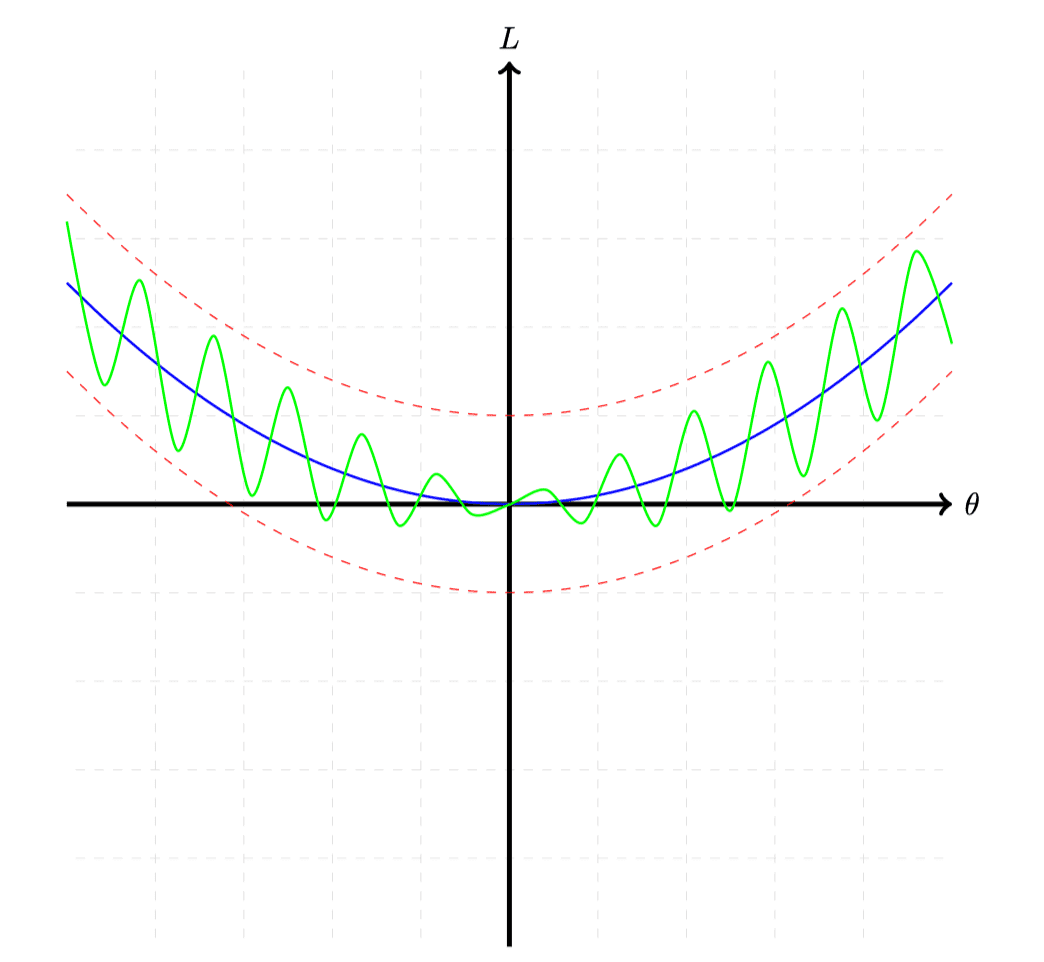
\includegraphics[width=\textwidth]{Figs/1.png}
         \caption{$y=x$}
         \label{fig:1}
     \end{subfigure}
     \hfill
     \begin{subfigure}[b]{0.47\textwidth}
         \centering
         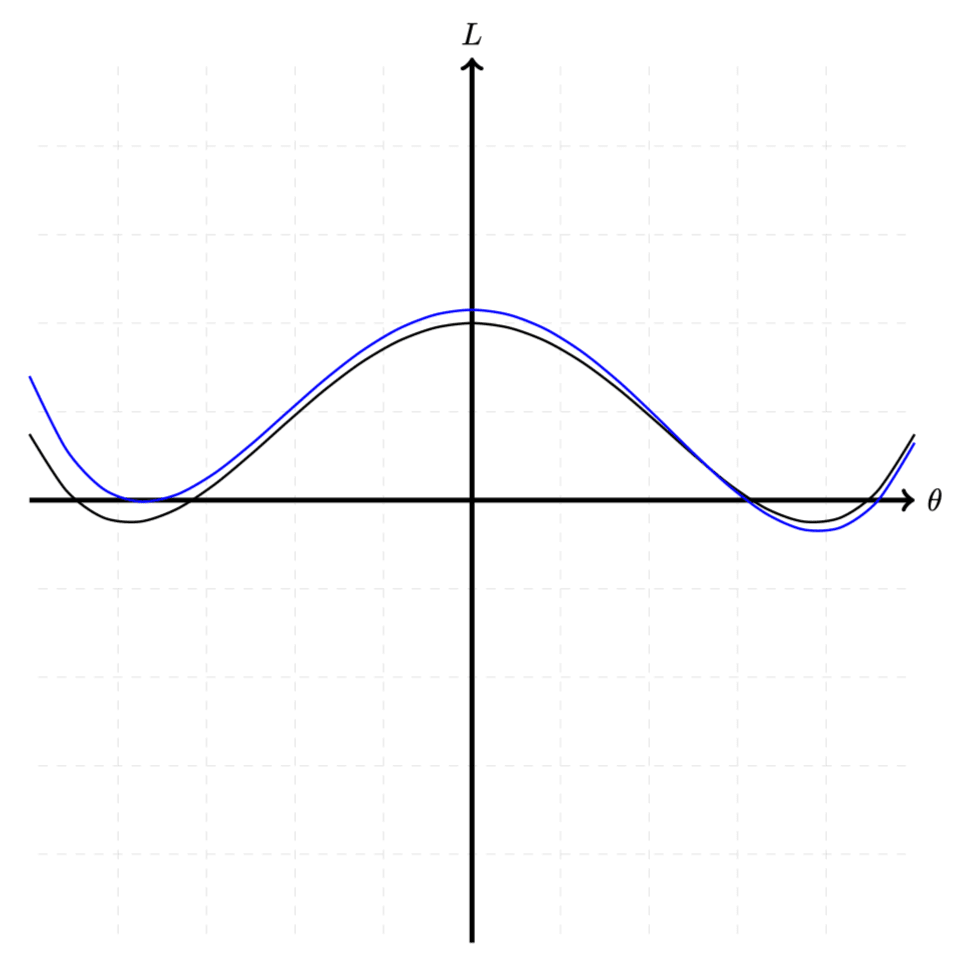
\includegraphics[width=\textwidth]{Figs/2.png}
         \caption{$y=3sinx$}
         \label{fig:2}
     \end{subfigure}
\end{figure}

\subsection{Finite Hypothesis Class}
$\bullet$ \tb{Assumption:}  $\mathcal{H}$ is finite, $0 \leq \ell((x, y), h) \leq 1$
\subsubsection{Main Theorem}
The following theorem gives a bound for the excess risk $L(\hat{h})-L\left(h^{*}\right)$ where $\hat{h}$ and $h^{*}$ are the minimizers of the empirical loss and population loss respectively.

\begin{thma}\label{thm:finite_uniform}
Suppose that our hypothesis class $\mathcal{H}$ is \tb{finite} and that our loss function $\ell$ is bounded in $[0,1]$. Then $\forall \delta$ s.t. $0<\delta<\frac{1}{2}$, with probability at least $1-\delta$, we have
\begin{align}
|L(h)-\hat{L}(h)| \leq \sqrt{\frac{\ln |\mathcal{H}|+\ln (2 / \delta)}{2 n}} \quad \forall h \in \mathcal{H}\label{eq:fda}
\end{align}
As a corollary, we also have
\begin{align}
L(\hat{h})-L\left(h^{*}\right) \leq \sqrt{\frac{2(\ln |\mathcal{H}|+\ln (2 / \delta))}{n}}\label{eq:hjfda}
\end{align}
\end{thma}
\begin{rema}\bfs{more explanation}\label{rem:qiied} Below are not that important, just for thinking. Here we have $\forall h\in \calH$, but normally when we consider $O_p$, we does not consider the uniform bound. I keep the following as my exercise.
\begin{enumerate}
    \item $\delta$ can be set as any $\omega(n)$ so $|L(h)-\hat{L}(h)|=O_p(\sqrt{\frac{\ln |\calH|}{n}}) \quad \forall h\in \calH$. 
    \item $\delta$ can be set as $n^{-\alpha}$ $\Rightarrow$ $|L(h)-\hat{L}(h)|\le \sqrt{\frac{\ln |\mathcal{H}|+C\ln n}{2 n}}=\ln n\sqrt{\frac{\ln |\mathcal{H}|}{2 n}}$, i.e. $\omega(n)=\ln n$
    \item why not set as $\alpha^{-n}$? of course can, but then $\alpha'^n\sqrt{\frac{\ln |\calH|}{n}}$ is not that useful.
    \item To directly get the $O_p$ order from \cref{eq:hfdafe} without referring \cref{eq:fda}, we can set $2|\mathcal{H}| \exp \left(-2 n \epsilon^{2}\right)=\frac{1}{\omega(n)}$, we have $\epsilon = \omega'(n)\sqrt{\frac{\ln |\calH|}{n}}$.
\end{enumerate}
\end{rema}
\begin{proof}
 We will prove this in two steps:
 \begin{enumerate}
     \item Use concentration inequalities to prove the bound for a fixed $h \in \mathcal{H}$, then
     \item Use a union bound across the $h$ 's. (Recall that if $E_{1}, \ldots, E_{k}$ are a finite set of events, then the union bound states that $\left.\operatorname{Pr}\left(E_{1} \cup \cdots \cup E_{k}\right) \leq \sum_{i=1}^{k} \operatorname{Pr}\left(E_{i}\right) .\right)$
 \end{enumerate}
Fix some $\epsilon>0 .$ By applying Hoeffding's inequality on the $\ell\left(\left(x^{(i)}, y^{(i)}\right), h\right)$, we know that
\begin{align*}
\begin{aligned}
\operatorname{Pr}(|\hat{L}(h)-L(h)| \geq \epsilon) & \leq 2 \exp \left(-\frac{2 n^{2} \epsilon^{2}}{\sum_{i=1}^{n}\left(b_{i}-a_{i}\right)^{2}}\right) \\
&=2 \exp \left(-\frac{2 n^{2} \epsilon^{2}}{n}\right) \\
&=2 \exp \left(-2 n \epsilon^{2}\right)
\end{aligned}
\end{align*}
since we can set $a_{i}=0, b_{i}=1$. The bound above holds for a single fixed $h$. To prove a similar inequality that holds for all $h \in \mathcal{H}$, we apply the union bound with $E_{h}=\{|\hat{L}(h)-L(h)| \geq \epsilon\}$ :
\begin{align}
\operatorname{Pr}(\exists h \text { s.t. }|\hat{L}(h)-L(h)| \geq \epsilon) & \leq \sum_{h \in \mathcal{H}} \operatorname{Pr}(|\hat{L}(h)-L(h)| \geq \epsilon) \nn
& \leq \sum_{h \in \mathcal{H}} 2 \exp \left(-2 n \epsilon^{2}\right) \nn
&=2|\mathcal{H}| \exp \left(-2 n \epsilon^{2}\right)\label{eq:hfdafe}
\end{align}
If we take $\delta$ such that $2|\mathcal{H}| \exp \left(-2 n \epsilon^{2}\right)=\delta$, then it follows that
\begin{align*}
\epsilon=\sqrt{\frac{\ln |\mathcal{H}|+\ln (2 / \delta)}{2 n}}
\end{align*}
which proves \cref{eq:fda}. \cref{eq:hjfda} follows by the inequality \cref{eq:decomp} and taking $\epsilon=\sqrt{\frac{2(\ln |\mathcal{H}|+\ln (2 / \delta))}{n}}$ :
\begin{align*}
\begin{aligned}
\operatorname{Pr}\left(\left|L(\hat{h})-L\left(h^{*}\right)\right| \geq \epsilon\right) & \leq \operatorname{Pr}\left(2 \sup _{h \in \mathcal{H}}\left|L(\hat{h})-L\left(h^{*}\right)\right| \geq \epsilon\right) \\
& \leq 2|\mathcal{H}| \exp \left(-\frac{n \epsilon^{2}}{2}\right)
\end{aligned}
\end{align*}
\end{proof}
\subsubsection{Comparing with Standard Concentration Inequalities}
$\bullet$  With standard concentration inequalities, we have the following bound that depends on empirical risk:
\begin{align*}
\forall h \in \mathcal{H}, \quad w.h.p . \quad|\hat{L}(h)-L(h)| \leq \tilde{O}\left(\frac{1}{\sqrt{n}}\right)
\end{align*}
The bound here depends on each $h$.

$\bullet$ In contrast, the uniform convergence bound we obtain from \cref{eq:fda} is uniform over all $h \in \mathcal{H}$ :
\begin{align*}
w.h.p. \quad \forall h \in \mathcal{H}, \quad|\hat{L}(h)-L(h)| \leq \tilde{O}\left(\frac{\ln |\mathcal{H}|}{\sqrt{n}}\right)
\end{align*}
if we omit the $\ln (1 / \delta)$ factor . Hence, the extra $\ln |\mathcal{H}|$ term that depends on the size of our finite hypothesis family $\mathcal{H}$ can be viewed as a trade-off in order to make the bound uniform.

\begin{rema}
We can omit $\ln (1 / \delta)$ factor since $\ln (1 / \delta)$ is small in general if we take $\delta=\frac{1}{\text { poly }(n)}$.
\end{rema}

\subsubsection{Comparing   with Asymptotic Bounds}
We can also compare the bound in \cref{thm:finite_uniform} with our original asymptotic bound, namely,
\begin{align*}
L(\hat{h})-L\left(h^{*}\right) \leq \frac{c}{n}+o\left(n^{-1}\right)
\end{align*}
The $o\left(n^{-1}\right)$ term can vary significantly depending on the problem. For instance, both $n^{-2}$ and $p^{100} n^{-2}$ are $o\left(n^{-1}\right)$ but the second one converges much more slowly. With the new bound, there are no longer any constants hidden in an $o\left(n^{-1}\right)$ term (in fact that term is no longer there). However, we now have a slower convergence rate of $O\left(n^{-1 / 2}\right)$.
\begin{rema}\bfs{some explanation} Please note that 
\begin{enumerate}
    \item $O\left(n^{-1 / 2}\right)$ convergence is sometimes known as the \tb{slow rate} while $O\left(n^{-1}\right)$ convergence is known as the \tb{fast rate}.
    \item We were only able to get the slow rate from uniform convergence: we needed asymptotics to get the fast rate.
    \item It is possible to get the fast rate from uniform convergence under certain conditions, e.g. when the population risk on the true $h^{*}$ is very low.
\end{enumerate}
\end{rema}
\subsection{Bounds for Infinite Hypothesis Class via Discretization}
We consider a bounded and continuous parameterized space of $\mathcal{H}$, then we can obtain a similar uniform bound by applying a technique called \tb{brute-force discretization}.

$\bullet$ \tb{Assumption:} infinite hypothesis class $\mathcal{H}$ can be parameterized by $\theta \in \mathbb{R}^{p}$ with $\|\theta\|_{2} \leq B$ for some fixed $B>0$. That is, we have
\begin{align*}
\mathcal{H}=\left\{h_{\theta}: \theta \in \mathbb{R},\|\theta\|_{2} \leq B\right\}
\end{align*}

$\bullet$ \tb{Main Idea:}
\begin{enumerate}
    \item The union bound does not work as we end up with an infinite sum. However, the union bound is very loose: these events can overlap with each other significantly. 
    \item Instead, we can try to find "prototypical" bad events $E_{\theta_{1}}, \ldots, E_{\theta_{N}}$ that are somewhat \tb{disjoint} so that $\bigcup_{\theta} E_{\theta} \approx \bigcup_{i=1}^{N} E_{\theta_{i}} .$ We can then use the union bound on $\bigcup_{i=1}^{N} E_{\theta_{i}}$ to get a non-vacuous upper bound. 
    \item In other words, we find a finite cover of the ball.
\end{enumerate}
\subsubsection{Discretization of the Parameter Space by $\epsilon$-covers}
We start by defining the notion of an $\epsilon$-cover (also $\epsilon$-net):
\begin{defa}\bfs{$\epsilon$-cover}\label{def:hkjererqre}
 Let $\epsilon>0 .$ An $\epsilon$-cover of a set $S$ \gls{wrt} distance metric $\rho$ is a subset $C \subseteq S$ such that $\forall x \in S, \exists x^{\prime} \in C$ such that $\rho\left(x, x^{\prime}\right) \leq \epsilon$, or equivalently,
\begin{align*}
\begin{aligned}
S & \subseteq \bigcup_{x \in C} \operatorname{Ball}(x, \epsilon, \rho), \quad \text { where } \\
\operatorname{Ball}(x, \epsilon, \rho) & \triangleq\left\{x^{\prime}: \rho\left(x, x^{\prime}\right) \leq \epsilon\right\}
\end{aligned}
\end{align*}
\end{defa}

The following lemma tells us that our parameter space $S=\left\{\theta \in \mathbb{R}^{p}:\|\theta\|_{2} \leq B\right\}$ has an $\epsilon$-cover with not too many elements:

\begin{lema}\bfs{$\epsilon$-cover of $\ell_{2}$ ball)} \label{lem:cover}Let $B, \epsilon>0$ with $\epsilon \leq B \sqrt{p}$, and let $S=\left\{x \in \mathbb{R}^{p}:\|x\|_{2} \leq B\right\} .$ Then there exists an $\epsilon$-cover of $S$ \gls{wrt} the $\ell_{2}-n o r m$ with at most $\left(\frac{3 B \sqrt{p}}{\epsilon}\right)^{p}$ elements.
\end{lema}
\begin{proof}
  Set
\begin{align*}
C=\left\{x \in S: x_{i}=k_{i} \frac{\epsilon}{\sqrt{p}}, k_{i} \in \mathbb{Z},\left|k_{i}\right| \leq \frac{B \sqrt{p}}{\epsilon}\right\}
\end{align*}
i.e. $C$ is the set of grid points in $\mathbb{R}^{p}$ of width $\frac{\epsilon}{\sqrt{p}}$ that are contained in $S .$ See \cref{fig:cover} for an illustration.
We claim that $C$ is an $\epsilon$-cover of $S$ \gls{wrt} the $\ell_{2}$-norm: $\forall x \in S$, there exists a grid point $x^{\prime} \in C$ such that $\left|x_{i}-x_{i}^{\prime}\right| \leq \frac{\epsilon}{\sqrt{p}}$ for each $i .$ Therefore,
\begin{align*}
\left\|x-x^{\prime}\right\|_{2}=\sqrt{\sum_{i=1}^{p}\left|x_{i}-x_{i}^{\prime}\right|^{2}} \leq \sqrt{p \cdot \frac{\epsilon^{2}}{p}}=\epsilon
\end{align*}
We now bound the size of $C .$ Since each $k_{i}$ in the definition of $C$ has at most $2 \frac{B \sqrt{p}}{\epsilon}+1$ choices, we have
\begin{align*}
|C| \leq\left(\frac{2 B \sqrt{p}}{\epsilon}+1\right)^{p} \leq\left(\frac{3 B \sqrt{p}}{\epsilon}\right)^{p}
\end{align*}
\end{proof}
\begin{figure}
    \centering
    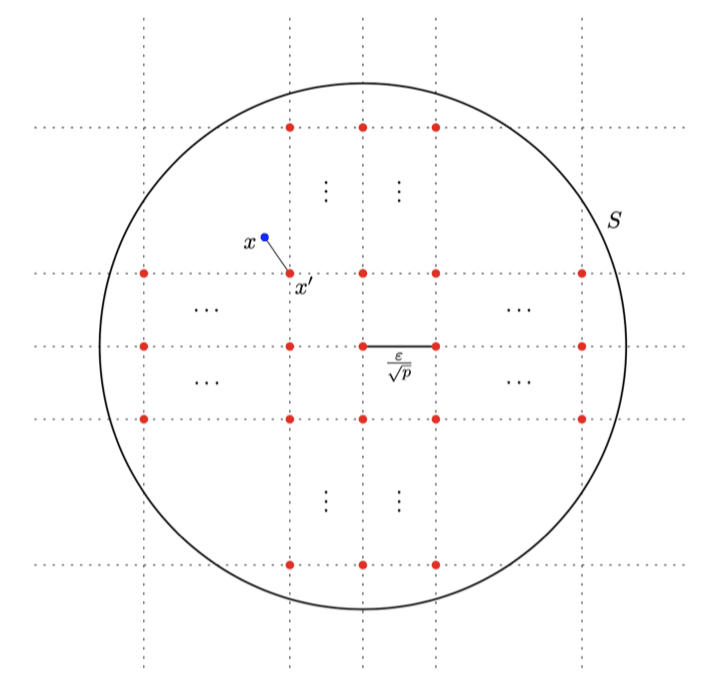
\includegraphics[width=0.7\textwidth]{Figs/3.png}
    \caption{Our chosen $\epsilon$-cover (shown in red) of $S .$ For $x \in S$, we choose the grid point $x^{\prime}$ such that $\left\|x-x^{\prime}\right\|_{2} \leq \epsilon$}
    \label{fig:cover}
\end{figure}
\begin{rema}\bfs{stronger version}
We can actually prove a stronger version of \cref{lem:cover}:

\tb{\centerline{There exists an $\epsilon$-cover of $S$ with at most $\left(\frac{3 B}{\epsilon}\right)^{p}$ elements.}}

We will be using this version of the lemma in the proof below. (I don't have time to prove this.)
\end{rema}
\subsubsection{Uniform Convergence Bound for Infinite $\calH$}
\begin{defa}\bfs{$\kappa$-Lipschitz functions}
  Let $\kappa \geq 0$ and $\|\cdot\|$ be a norm on the domain $D$. A function $L: D \rightarrow \mathbb{R}$ is said to be $\kappa$-Lipschitz \gls{wrt} $\|\cdot\|$ if for all $\theta, \theta^{\prime} \in D$, we have
\begin{align*}
\left|L(\theta)-L\left(\theta^{\prime}\right)\right| \leq \kappa\left\|\theta-\theta^{\prime}\right\|
\end{align*}
\end{defa}

\begin{thma}\label{thm:infinite_uniform}
Suppose $\ell((x, y), \theta) \in[0,1]$, and $\ell((x, y), \theta)$ is $\kappa$-Lipschitz in $\theta$ \gls{wrt} the $\ell_{2}$-norm for all $(x, y)$. Then, with probability at least $1-O(\exp (-\Omega(p)))$, we have 
\begin{align*}
\forall \theta, \quad|\hat{L}(\theta)-L(\theta)| \leq O\left(\sqrt{\frac{p \max (\ln (\kappa B n), 1)}{n}}\right)
\end{align*}
\end{thma}
\begin{rema}\bfs{explanation}
\begin{enumerate}
    \item $O(\exp (-\Omega(p))$ can of course be set as other order like $O(\ln (-p))$, and we can a smaller order than $O\left(\sqrt{\frac{p \max (\ln (\kappa B n), 1)}{n}}\right)$. But from \cref{eq:hkz1}, we know the improvement is not that much and we still have $O\left(\sqrt{\frac{(p/\ln p) \max (\ln (\kappa B n), 1)}{n}}\right)$.
    \item Compare to \cref{rem:qiied} and \cref{thm:finite_uniform}, where is $n$? why only $O(\exp (-\Omega(p)))$ is shown here.  From \cref{eq:mxnbdee} we can see the dependence on $n$. The full one should be $O\big(\exp (-\Omega(p)\ln n)\big)$, which is polynomial on $n$.  Roughly speakly, with high probability we have \begin{align*}
\forall \theta, \quad|\hat{L}(\theta)-L(\theta)| \leq O\left(\sqrt{\frac{p}{n}}\right)
\end{align*}
    \item See  \cref{rema:gujjda} part 1. for more thinking.
\end{enumerate}

\end{rema}
\begin{proof}
  Fix parameters $\delta, \epsilon>0$ (we will specify their values later). Let $C$ be the $\epsilon$-cover of our parameter space $S$ \gls{wrt} the $\ell_{2}$-norm constructed in \cref{lem:cover}. Define event $E=$ $\{\forall \theta \in C,|\hat{L}(\theta)-L(\theta)| \leq \delta\} .$ By \cref{thm:finite_uniform}, we have $\operatorname{Pr}(E) \geq 1-2|C| \exp \left(-2 n \delta^{2}\right)$

Now for any $\theta \in S$, we can pick some $\theta_{0} \in C$ such that $\left\|\theta-\theta_{0}\right\|_{2} \leq \epsilon$. Since $L$ and $\widehat{L}$ are $\kappa$-Lipschitz functions (this follows from the Lipschitzness of $\ell$ ), we have
\begin{align*}
\begin{aligned}
&\left|L(\theta)-L\left(\theta_{0}\right)\right| \leq \kappa\left\|\theta-\theta_{0}\right\|_{2} \leq \kappa \epsilon, \text { and } \\
&\left|\hat{L}(\theta)-\hat{L}\left(\theta_{0}\right)\right| \leq \kappa\left\|\theta-\theta_{0}\right\|_{2} \leq \kappa \epsilon
\end{aligned}
\end{align*}
Therefore, conditional on $E$, we have
\begin{align*}
|\hat{L}(\theta)-L(\theta)| \leq\left|\hat{L}(\theta)-\hat{L}\left(\theta_{0}\right)\right|+\left|\hat{L}\left(\theta_{0}\right)-L\left(\theta_{0}\right)\right|+\left|L\left(\theta_{0}\right)-L(\theta)\right| \leq 2 \kappa \epsilon+\delta
\end{align*}
It remains to choose suitable parameters $\delta$ and $\epsilon$ to get the desired bound in \cref{thm:infinite_uniform} while making the failure probability small. First, set $\epsilon=\delta /(2 \kappa)$ so that conditional on $E$,
\begin{align}
|\hat{L}(\theta)-L(\theta)| \leq 2 \delta .\label{eq:hnieqd}
\end{align}

If we set $\delta=\sqrt{\frac{c_{0} p \max (1, \ln (\kappa B n))}{n}}$ with $c_{0}=36$ (see \cref{rema:ghyfd} for some intuition), then
\begin{align}
\ln |C|-2 n \delta^{2} & \leq p \ln \left(\frac{6 B \kappa}{\delta}\right)-2 n \delta^{2} \label{eq:hkz1}\\
& \leq p \ln \left(\frac{6 B \kappa \sqrt{n}}{\sqrt{c_{0} p \max (1, \ln (\kappa B n))}}\right)-2 n \frac{c_{0} p}{n} \ln (\kappa B n) \\
& \leq p \ln \left(\frac{B \kappa \sqrt{n}}{\sqrt{p}}\right)-72 p \ln (\kappa B n) \\
& \leq p \ln (B \kappa n)-72 p \ln (B \kappa n) \label{eq:mxnbdee}\\
& \leq-p
\end{align}
since $\ln (B \kappa n) \geq 1$ for large enough $n .$ Therefore, with probability greater than $1-2|C| \exp \left(-2 n \delta^{2}\right)=$ $1-2 \exp \left(\ln |C|-2 n \delta^{2}\right) \geq 1-O\left(e^{-p}\right)$, we have
\begin{align*}
|\hat{L}(\theta)-L(\theta)| \leq 2 \delta=O\left(\sqrt{\frac{p}{n} \max (1, \ln (\kappa B n))}\right)
\end{align*}
\end{proof}
\begin{rema}\label{rema:ghyfd}\bfs{ intuition for the choice of $\delta$} The event $E$ happens with probability $1-2|C| \exp \left(-2 n \delta^{2}\right)=1-2 \exp \left(\ln |C|-2 n \delta^{2}\right) .$ We know that $\ln |C| \leq p \ln (3 B /\epsilon)$. If we ignore the $\ln$ term and assume $\ln | C| \leq p$, then this would give us the high probability bound we want:
\begin{align*}
2|C| \exp \left(-2 n \delta^{2}\right)=2 \exp \left(\ln |C|-2 n \delta^{2}\right) \leq 2 \exp (p-2 p)=2 \exp (-p)
\end{align*}
At the same time, we see from \cref{eq:hnieqd} that this choice of $\delta$ gives $|\hat{L}(\theta)-L(\theta)| \leq 2 \sqrt{\frac{p}{n}}$, which is roughly the bound we want.

Since we cannot drop the log term in the inequality, we need to make $\delta$ a little big bigger. $\delta$ in the proof was chosen with this intuition in mind to make the subsequent chain of logic work.
\end{rema} 
\begin{rema}\label{rema:gujjda}
\begin{enumerate}
    \item We bounded the generalization error $|\hat{L}(\theta)-L(\theta)|$ by $\delta+2 \epsilon \kappa \leq \sqrt{\frac{\ln |C|}{n}}+2 \epsilon \kappa .$ The term $2 \epsilon \kappa$ represents the error from our brute-force discretization. It is not a problem is because we can always choose $\epsilon$ small enough without worrying about the growth of the first term $\sqrt{\frac{\ln |C|}{n}}$. This in turn is because $\ln |C| \approx p \ln \epsilon^{-1}$, which is very \tb{insensitive} to $\epsilon$, even if we let $\epsilon=\frac{1}{\text { poly }(n)}$. 
    \item We also observe that both $\sqrt{\frac{\ln |C|}{n}}$ and $\sqrt{\frac{p}{n}}$ are bounds that depend on the "size" of our hypothesis class, in terms of either its total size or dimensionality. This possibly explains why one may need more training samples when the hypothesis class is larger.
\end{enumerate}
\end{rema} 

\subsection{Rademacher Complexity}
\subsubsection{Motivation for A New Complexity Measure}
In the previous sections, we derived bounds for the generalization gap in two cases:
\begin{itemize}
    \item If the hypothesis class $\mathcal{H}$ is finite,
\begin{align*}
L(\hat{h})-\hat{L}(\hat{h}) \leq \tilde{O}\left(\sqrt{\frac{\log |\mathcal{H}|}{n}}\right)
\end{align*}
\item If the hypothesis class $\mathcal{H}$ is $p$-dimensional,
\begin{align}
L(\hat{h})-\hat{L}(\hat{h}) \leq \tilde{O}\left(\sqrt{\frac{p}{n}}\right)\label{eq:hmjdq}
\end{align}
\end{itemize}
Both of these bounds have a $\frac{1}{\sqrt{n}}$-dependency on $n$, which is known as the "slow rate". The terms in the numerator $(\log |\mathcal{H}|$ and $p$ resp. $)$ can be thought of as \tb{complexity measure} of $\mathcal{H}$.

$\bullet$ \tb{Drawback:} 

The bound \cref{eq:hmjdq} is not precise enough: it depends solely on $p$ and is not always optimal. For example, this would be a poor bound if the hypothesis class $\mathcal{H}$ has very high dimension but small norm. 

$\bullet$ \tb{New Objective:} 

With the complexity measure to be introduced, we will prove a bound of the form
\begin{align*}
L(\hat{h})-\hat{L}(\hat{h}) \leq \tilde{O}\left(\sqrt{\frac{\operatorname{Complexity}(\Theta)}{n}}\right)
\end{align*}
This complexity measure will depend on the distribution $P$ over $\mathcal{X} \times \mathcal{Y}$ (the input and output spaces), and hence takes into account how easy it is to learn $P$. If $P$ is easy to learn, then this complexity measure will be small even if the hypothesis space is big.
\begin{rema}\bfs{complexity measure as regularizer}
One of the practical implications of having such a complexity measure is that we can restrict the hypothesis space by regularizing the complexity measure (assuming it is something we can evaluate and train with). If we successfully find a low complexity model, then this generalization bound guarantees that we have not overfit.
\end{rema}
$\bullet$ \tb{Some Difference between The Uniform Convergence and The Bounds in This Section:} 

\begin{itemize}
    \item In uniform convergence, we sought a high probability bound for $\sup _{h \in H}(L(h)-\hat{L}(h))$. 
    \item Here we first take a weaker form in \cref{sssec:gmrdrfer}: we try to obtain an upper bound for its expectation instead, i.e.
\begin{align*}
\mathbb{E}_{z \sim X \times Y}\left[\sup _{h \in H}(L(h)-\hat{L}(h))\right] \leq \text { upper bound. }
\end{align*}
The expectation is over the randomness in the training data $(\mathcal{X} \times \mathcal{Y})$. (Note: We cannot just swap the order of $\mathbb{E}$ and sup!)
\item For uniform convergence bound, see \cref{eq:nierfa}.
\end{itemize}

To do so, we first define Rademacher complexity.
\subsubsection{Definitions}

\begin{defa}\bfs{Rademacher Complexity}
  Let $\mathcal{F}$ be a family of functions mapping $Z \mapsto \mathbb{R}$, and let $P$ be a distribution over $Z$. The \tb{Rademacher complexity} of $\mathcal{F}$ is defined as
  \begin{align}
      R_{n}(F) \triangleq \mathbb{E}_{z_{1}, \ldots, z_{n} \stackrel{\mathrm{iid}}{\sim} P}\left[\mathbb{E}_{\sigma_{1}, \ldots, \sigma_{n}\stackrel{\mathrm{iid}}{\sim}\{\pm 1\}} \left[\sup _{f \in F} \frac{1}{n} \sum_{i=1}^{n} \sigma_{i} f\left(z_{i}\right)\right]\right]
  \end{align}
where $\sigma_{1}, \ldots, \sigma_{n}$ are independent Rademacher random variables, i.e. each taking on the value of 1 or $-1$ with probability $1 / 2$.
\end{defa}



\begin{rema}\text{ \\}
\begin{enumerate}
    \item For our applications we will take $\mathcal{Z}=\mathcal{X} \times \mathcal{Y}$. However, Definition $4.12$ holds for abstract input spaces $\mathcal{Z}$ as well.
    \item Note that $R_{n}(\mathcal{F})$  \tb{is dependent on the measure $P$ of the space and the hypothesis space $\calF$,} so technically it should be $R_{n, P}(\mathcal{F})$, but for brevity, we refer to it as $R_{n}(\mathcal{F})$.
\end{enumerate}
\end{rema}

\begin{defa}\bfs{Empirical Rademacher complexity}
 Given a dataset $S=\left\{z_{1}, \ldots, z_{n}\right\}$, the emprical Rademacher complexity is defined as
\begin{align*}
R_{S}(\mathcal{F}) \triangleq \mathbb{E}_{\sigma_{1}, \ldots, \sigma_{n}}\left[\sup _{f \in \mathcal{F}} \frac{1}{n} \sum_{i=1}^{n} \sigma_{i} f\left(z_{i}\right)\right]
\end{align*}
\end{defa}
\begin{rema}\text{ \\}
\begin{enumerate}
    \item $R_{S}(\mathcal{F})$ is a function of both the function class $\mathcal{F}$ and the dataset $S$. More specifically, it  \tb{is dependent on one sampled set $\calQ_{\calF}$ \gls{wrt} $P$ and $\calF$, i.e. the set $\calQ_\calF = \{[f(z_1),...,f(z_n)]\mid f \in \calF\}$.} See also \cref{sssect:empri_rad_com}.
    \item The expectation of the empirical Rademacher complexity is the Rademacher complexity:
    $$R_{n}(\mathcal{F})=\underset{z_{1}, \ldots, z_{n} \stackrel{\operatorname{iid}}{\sim} P \atop S=\left\{z_{1}, \ldots, z_{n}\right\}}{\mathbb{E}}\left[R_{S}(\mathcal{F})\right]$$
\end{enumerate}
\end{rema}




\begin{rema}\bfs{What does Rademacher complexity mean?}\\
Intuitively, the supremum measures, for a given set $S$ and Rademacher vector $\sigma$, the maximum correlation between $f\left(z_{i}\right)$ and $\sigma_{i}$ over all $f \in \mathcal{F}$. Essentially, functions with more random sign outputs will better match random patterns of Rademacher vector and have higher complexity (greater ability to mimic or express randomness).
\begin{enumerate}
    \item Taking the expectation over $\sigma$, we can then say that the \tb{empirical Rademacher complexity} of $\mathcal{F}$ measures the ability of functions from $\mathcal{F}$ (when applied to a fixed set $S$ ) to fit random noise.
    \item The \tb{Rademacher complexity} of $\mathcal{F}$ then measures the expected noise-fitting-ability of $\mathcal{F}$ over all data sets $S \in Z^{m}$ that could be drawn according to the distribution $P$.
\end{enumerate}
\end{rema}

\subsubsection{Bounds using Rademacher complexity}\label{sssec:gmrdrfer}
\begin{thma}\bfs{Rademacher Complexity Bound}\label{thma:gndafaxv}
\begin{align}
\mathbb{E}_{z_{1}, \ldots, z_{n}{\stackrel{\mathrm{iid}}{\sim}}P} \left[\sup _{f \in F}\left[\frac{1}{n} \sum_{i=1}^{n} f\left(z_{i}\right)-\mathbb{E}_{z \sim P} f(x)\right]\right] \leq 2 R_{n}(\mathcal{F})\label{eq:mrire3e}
\end{align}
\end{thma}

\begin{rema}\bfs{explanation}
We can think of $\frac{1}{n} \sum_{i=1}^{n} f\left(z_{i}\right)$ as an empirical average and $\mathbb{E}_{z \sim P} f(x)$ as a population average. Here is an intuitive understanding of what \cref{thma:gndafaxv}  achieves. Consider the quantities on the LHS and RHS of \cref{eq:mrire3e}:
\begin{align*}
\sup _{f \in \mathcal{F}}\left(\frac{1}{n} \sum_{i=1}^{n} f\left(z_{i}\right)-\mathbb{E}[f]\right) \quad \text { v.s. } \quad \sup _{f \in \mathcal{F}}\left(\frac{1}{n} \sum_{i=1}^{n} \sigma_{i} f\left(z_{i}\right)\right)
\end{align*}

\begin{itemize}
    \item First, we removed $\mathbb{E}[f]$, which is hard to control quantitatively since $f$ is deterministic. 
    \item Second, we added more randomness using the form of Rademacher variables. This will allow us to shift our focus from the randomness in the $z_{i}$ 's to the randomness in the $\sigma_{i}$ 's.
    \item  In the future, our bounds on the empirical Rademacher complexity will typically only depend on the randomness from the $\sigma_{i}$ 's.
\end{itemize}
\end{rema}


\begin{proof}
 We use a technique called \tb{symmetrization}, which is a very important technique in probability theory. We first fix $z_{1}, \ldots, z_{n}$ and draw $z_{1}^{\prime}, \ldots z_{n}^{\prime} \stackrel{\text { iid }}{\sim} P .$ Then we can rewrite the term in the expectation on the LHS of \cref{eq:mrire3e}:
\begin{align*}
\begin{aligned}
\sup _{f \in \mathcal{F}}\left(\frac{1}{n} \sum_{i=1}^{n} f\left(z_{i}\right)-\mathbb{E}[f]\right) &=\sup _{f \in \mathcal{F}}\left(\frac{1}{n} \sum_{i=1}^{n} f\left(z_{i}\right)-\mathbb{E}_{z_{1}^{\prime}, \ldots, z_{n}^{\prime}}\left[\frac{1}{n} \sum_{i=1}^{n} f\left(z_{i}^{\prime}\right)\right]\right) \\
&=\sup _{f \in \mathcal{F}}\left(\mathbb{E}_{z_{1}^{\prime}, \ldots, z_{n}^{\prime}}\left[\frac{1}{n} \sum_{i=1}^{n} f\left(z_{i}\right)-\frac{1}{n} \sum_{i=1}^{n} f\left(z_{i}^{\prime}\right)\right]\right) \\
& \leq \mathbb{E}_{z_{1}^{\prime}, \ldots, z_{n}^{\prime}}\left[\sup _{f \in \mathcal{F}}\left(\frac{1}{n} \sum_{i=1}^{n} f\left(z_{i}\right)-\frac{1}{n} \sum_{i=1}^{n} f\left(z_{i}^{\prime}\right)\right)\right]
\end{aligned}
\end{align*}
The last inequality is because in general (not restrict to convex function),
\begin{align*}
\sup _{u}\left(\mathbb{E}_{v}[g(u, v)]\right) \leq \sup _{u}\left(\mathbb{E}_{v}\left[\sup _{u^{\prime}} g\left(u^{\prime}, v\right)\right]\right)=\mathbb{E}_{v}\left[\sup _{u}(g(u, v))\right]
\end{align*}
since the outer sup becomes vacuous.
Now, if we take the expectation over $z_{1}, \ldots, z_{n}$ for both sides of
\begin{align*}
\mathbb{E}_{z_{1}, \ldots, z_{n}}\left[\sup _{f \in \mathcal{F}}\left(\frac{1}{n} \sum_{i=1}^{n} f\left(z_{i}\right)-\mathbb{E}[f]\right)\right] & \leq \mathbb{E}_{z_{i}}\left[\mathbb{E}_{z_{i}^{\prime}}\left[\sup _{f \in \mathcal{F}}\left(\frac{1}{n} \sum_{i=1}^{n}\left(f\left(z_{i}\right)-f\left(z_{i}^{\prime}\right)\right)\right)\right]\right] \nn
&=\mathbb{E}_{z_{i}, z_{i}^{\prime}}\left[\mathbb{E}_{\sigma_{i}}\left[\sup _{f \in \mathcal{F}}\left(\frac{1}{n} \sum_{i=1}^{n} \sigma_{i}\left(f\left(z_{i}\right)-f\left(z_{i}^{\prime}\right)\right)\right)\right]\right] \\
& \leq \mathbb{E}_{z_{i}, z_{i}^{\prime}, \sigma_{i}}\left[\sup _{f \in \mathcal{F}}\left(\frac{1}{n} \sum_{i=1}^{n} \sigma_{i} f\left(z_{i}\right)\right)+\sup _{f \in \mathcal{F}}\left(\frac{1}{n} \sum_{i=1}^{n}-\sigma_{i} f\left(z_{i}^{\prime}\right)\right)\right] \nn
&=2 R_{n}(\mathcal{F})\nn
\end{align*}
where the second equality is because $\sigma_{i}\left(f\left(z_{i}\right)-f\left(z_{i}^{\prime}\right)\right) \stackrel{d}{=} f\left(z_{i}\right)-f\left(z_{i}^{\prime}\right)$ since $f\left(z_{i}\right)-f\left(z_{i}^{\prime}\right)$ has a symmetric distribution. The last equality holds since $-\sigma_{i} \stackrel{d}{=} \sigma_{i}$ and $z_{i}, z_{i}^{\prime}$ are drawn \gls{iid} from the same distribution.
\end{proof}
\begin{cora}\bfs{apply \cref{thma:gndafaxv} to bound average generalization error (weak form)}
 We can set $\mathcal{F}$ to be the family of loss functions, i.e.
\begin{align*}
\mathcal{F}=\{z=(x, y) \in \mathcal{Z} \mapsto \ell((x, y), h) \in \mathbb{R}: h \in \mathcal{H}\}
\end{align*}
This is the family of losses induced from the hypothesis functions in $\mathcal{H}$. Then by \cref{thma:gndafaxv}
\begin{align*}
\begin{aligned}
\mathbb{E}_{\{z_{i}\}}\left[\sup _{f \in F}\left(\frac{1}{n} \sum_{i=1}^{n} f\left(z_{i}\right)-\mathbb{E}(f)\right)\right] &=\mathbb{E}_{\{\left(x^{(i)}, y^{(i)}\right)\}}\left[\sup _{h \in \mathcal{H}}\left[\frac{1}{n} \sum_{i=1}^{n} \ell\left(\left(x^{(i)}, y^{(i)}, h\right)\right)-L(h)\right]\right] \\
&=\mathbb{E}\left[\sup _{h \in \mathcal{H}}(\hat{L}(h)-L(h))\right] \\
& \leq 2 R_{n}(\mathcal{F})
\end{aligned}
\end{align*}
where $z_{i}=\left(x^{(i)}, y^{(i)}\right)$. Thus, $2 R_{n}(\mathcal{F})$ is an upper bound for the generalization error. In this context, $R_{n}(\mathcal{F})$ can be interpreted as how well the loss sequence $\ell\left(\left(x^{(1)}, y^{(1)}\right), h\right), \ldots \ell\left(\left(x^{(n)}, y^{(n)}\right), h\right)$ correlates with $\sigma_{1}, \ldots, \sigma_{n}$
\end{cora}
\begin{rema}\bfs{strong form (uniform convergence)}
For high probability bound of generalization error (not expectation) see \cref{eq:hererqrewytr} where get with probability $1-\delta$, we have
\begin{align}
L(h)-\hat{L}(h) \leq 2 R_{n}(F)+\sqrt{\frac{\log (2 / \delta)}{2 n}} \quad \text { for all } h \in \mathcal{H}
\end{align}
\end{rema}

\subsubsection{Special Case: Moving from $\mathcal{R}_{s}(\mathcal{F})$ to $\mathcal{R}_{s}(\mathcal{H})$}

$\bullet$ \tb{One special case:}

\begin{exma}
Consider the binary classification setting where $y \in\{\pm 1\} .$ Let $\ell_{0-1}$ denote the zero-one loss function (\tb{not Lipschitz, a relaxation is shown in \cref{exma:gdrtqe}}). Note that
\begin{align*}
\ell_{0-1}((x, y), h)=\mathbf{1}\{h(x) \neq y\}=\frac{1-y h(x)}{2}
\end{align*}
Hence,
\begin{align*}
R_{n}(\mathcal{F})=& \mathbb{E}_{\left(x^{(i)}, y^{(i)}\right), \sigma_{i}}\left[\sup _{h \in \mathcal{H}} \frac{1}{n} \sum_{i=1}^{n} \ell_{0-1}\left(\left(x^{(i)}, y^{(i)}\right), h\right) \sigma_{i}\right] \\
=& \mathbb{E}_{\left(x^{(i)}, y^{(i)}\right), \sigma_{i}}\left[\sup _{h \in \mathcal{H}} \frac{1}{n} \sum_{i=1}^{n}\left(\frac{-h\left(x^{(i)}\right) y^{(i)}+1}{2}\right) \sigma_{i}\right] \\
=&\frac{1}{2} \mathbb{E}_{\left(x^{(i)}, y^{(i)}\right), \sigma_{i}} \left[\frac{1}{n} \sum_{i=1}^{n} \sigma_{i}+\sup _{h \in \mathcal{H}} \frac{1}{n} \sum_{i=1}^{n}-h\left(x^{(i)}\right) y^{(i)} \sigma_{i}\right] \\
=&\frac{1}{2} \mathbb{E}_{\left(x^{(i)}, y^{(i)}\right), \sigma_{i}}\left[\sup _{h \in \mathcal{H}} \frac{1}{n} \sum_{i=1}^{n}-h\left(x^{(i)}\right) y^{(i)} \sigma_{i}\right] \\
=&\frac{1}{2} \mathbb{E}_{\left(x^{(i)}, y^{(i)}\right), \sigma_{i}} \left[\sup _{h \in \mathcal{H}} \frac{1}{n} \sum_{i=1}^{n} h\left(x^{(i)}\right) \sigma_{i}\right] \quad \text{since  $\left(-y_{i} \sigma_{i} \stackrel{d}{=} \sigma_{i}\right)$}\\
=&\frac{1}{2} R_{n}(\mathcal{H}) 
\end{align*}
In this setting, $R_{n}(\mathcal{F})$ and $R_{n}(\mathcal{H})$ are the same (except for the factor of 2$) . R_{n}(\mathcal{H})$ has a slightly more intuitive interpretation: it represents how well $h \in \mathcal{H}$ can fit random patterns.
\end{exma} 
\begin{rema}\text{ \\}
\begin{enumerate}
    \item Warning! $R_{n}(\mathcal{F})$ is not always the same as $R_{n}(\mathcal{H})$ in other problems.
    \item Rademacher complexity is \tb{invariant to translation.} One example of this in play is in how the $+1$ in the $\left(\frac{-h\left(x^{(i)}\right) y^{(i)}+1}{2}\right)$ term essentially vanishes in the computation.
\end{enumerate}
\end{rema}

$\bullet$ \tb{General case using Lipschitz:}

\begin{lema}\bfs{Talagrand's Lemma (contraction principle and Lipschitz composition}
 Let $\phi: \mathbb{R} \mapsto \mathbb{R}$ be a $k$-Lipschitz function, then
\begin{align*}
\mathcal{R}_{s}(\phi \circ \mathcal{H}) \leq k \cdot \mathcal{R}_{s}(\mathcal{H})
\end{align*}
where $\phi \circ \mathcal{H}=\{z \mapsto \phi(h(z)): h \in \mathcal{H}\}$
\end{lema}


Consider a family of loss functions $\mathcal{F}=\{z \mapsto \ell((x, y), h): h \in \mathcal{H}\}$ where $\ell((x, y), h)$ can be expressed as
\begin{align*}
\ell((x, y), h)=\ell(h(x), y)
\end{align*}
Then, we can use Talagrand's lemma to \tb{remove the influence of the loss function.} Concretely, instead of the Rademacher complexity of the family of functions $\mathcal{F}$, we can derive a bound that depends on the Rademacher complexity of the hypothesis class $\mathcal{H}$. 

To be concrete, let us consider binary classification where $y_{i} \sim\{-1,+1\}$ together with two losses - hinge loss and binary loss.

\begin{exma}\bfs{Hinge Loss}
For hinge loss, we have
\begin{align*}
\ell(z, h)=\max \left(0,1-y_{i} h\left(x_{i}\right)\right)
\end{align*}
The hinge loss is 1-lipschitz. Let us define $\phi(t)=\max (0,1-t)$. Then, we have
\begin{align*}
\begin{aligned}
\mathcal{R}_{s}(\mathcal{F}) &=\underset{\sigma}{\mathbb{E}} \sup _{h \in \mathcal{H}} \frac{1}{n} \sum_{i=1}^{n} \sigma_{i} \phi\left(y_{i} h\left(x_{i}\right)\right) \\
& \leq \underset{\sigma}{\mathbb{E}} \sup _{h \in \mathcal{H}} \frac{1}{n} \sum_{i=1}^{n} \sigma_{i} y_{i} h\left(x_{i}\right) \\
&=\underset{\sigma}{\mathbb{E}} \sup _{h \in \mathcal{H}} \frac{1}{n} \sum_{i=1}^{n} \sigma_{i} h\left(x_{i}\right) \\
&=\mathcal{R}(\mathcal{H})
\end{aligned}
\end{align*}
where the inequality holds true because $\mathcal{F}=\phi \circ \mathcal{H}^{\prime}$ and by Talagrand, we have
\begin{align*}
\mathcal{R}_{s}(\mathcal{F}) \leq k \mathcal{R}_{s}\left(\mathcal{H}^{\prime}\right)
\end{align*}
where $\mathcal{H}^{\prime}=\{z \mapsto y h(x): h \in \mathcal{H}\} .$ Since hinge loss is 1-lipschitz, $k=1$
In the third step of the derivation, we can remove $y_{i}$ because $\sigma_{i}$ and $\sigma_{i} y_{i}$ come from the same distribution.
\end{exma} 

\begin{exma}\bfs{Binary Loss}\label{exma:gdrtqe}
Since binary loss is not Lipschitz, we use margin theory to upper bound the binary loss. We define the following \tb{$\gamma$-margin loss} for $\gamma>0$
\begin{align*}
\ell_{\gamma}(t)= \begin{cases}0, & \text { if } t \geq \gamma \\ 1, & \text { if } t \leq 0 \\ 1-\frac{t}{\gamma}, & \text { otherwise }\end{cases}
\end{align*}
Also let
\begin{align*}
\begin{gathered}
\ell_{\gamma}((x, y), h)=\ell_{\gamma}(y h(x)) \\
\mathcal{F}_{\gamma}=\left\{(x, y) \mapsto \ell_{\gamma}(y h(x))\right\}
\end{gathered}
\end{align*}
with $L_{\gamma}$ and $\hat{L}_{\gamma}$ defined accordingly.
We desire to give an upper bound on the expected binary loss. We give this bound by first giving bounds for the following three terms: $L(h), \hat{L}_{\gamma}(h)$ and $\left|\hat{L}_{\gamma}(h)-L_{\gamma}(h)\right|$.

\tb{Firstly}, notice that $\ell_{\gamma}$ upper-bounds the binary loss as shown below:
\begin{align*}
L(h)=\mathbb{E}[\mathbf{1}[y h(x)<0]] \leq \mathbb{E}\left[l_{\gamma}((x, y), h)\right]=L_{\gamma}(h)
\end{align*}
\tb{Secondly}, we bound $\hat{L}_{\gamma}(h)$ by the training loss w.r.t a margin. Intuitively, the training loss w.r.t. a margin means that a point is considered to be classified wrongly $(\ell=1)$ even if it is on the correct side of the decision boundary if the point is within $\gamma$ of the margin.
\begin{align*}
\hat{L}_{\gamma}(h)=\frac{1}{n} \sum_{i=1}^{n} \ell_{\gamma}\left(y_{i} h\left(x_{i}\right)\right) \leq \frac{1}{n} \sum_{i=1}^{n} \mathbf{1}\left[y_{i} h\left(x_{i}\right) \leq \gamma\right]
\end{align*}
\tb{Lastly}, we bound the generalization error of $\gamma$-margin loss: w.p $\geq 1-\delta$,
\begin{align*} \forall h,\left|\hat{L}_{\gamma}(h)-L_{\gamma}(h)\right| & \lesssim \mathcal{R}_{S}\left(\mathcal{F}_{\gamma}\right)+\sqrt{\frac{\log (2 / \delta)}{n}} \\ & \lesssim \frac{1}{\gamma} \mathcal{R}_{S}(\mathcal{H})+\sqrt{\frac{\log (2 / \delta)}{n}} \quad \text { by Talagrand's Lemma } 
\end{align*}

In particular, this implies the following:
\begin{align*}
L_{\gamma}(h) \lesssim \hat{L}_{\gamma}(h)+\frac{1}{\gamma} \mathcal{R}_{S}(\mathcal{H})+\sqrt{\frac{\log (2 / \delta)}{n}}
\end{align*}
Combining three inequalities, we obtain:
\begin{align*}
L(h) \leq \hat{L}_{\gamma}(h)+O\left(\frac{\mathcal{R}_{S}(\mathcal{H})}{\gamma}+\sqrt{\frac{\log (2 / \delta)}{n}}\right)
\end{align*}
Notice that the above inequality suggests a tradeoff in the choice of $\gamma$. For a large $\gamma$, the training loss w.r.t. a margin increases but the term on the right decreases and vice versa.
\end{exma} 



\subsubsection{Special Case: Upper Bound of Rademacher Complexity regardless of $\calF$}\label{eq:nierfa}
$\bullet$ \tb{Assumption: } $-1 \leq f\left(z_{0}\right) \leq 1$ for all $f \in \mathcal{F}$. $P$ is a point mass, i.e. $z = z_0$ almost surely.

\begin{align*}
\begin{aligned}
\mathbb{E}_{z_{1}, \ldots, z_{n} \sim P}\mathbb{E}_{\sigma_{1}, \ldots, \sigma_{n}}\left[\sup _{f \in \mathcal{F}} \frac{1}{n} \sum_{i=1}^{n} \sigma_{i} f\left(z_{i}\right)\right] &=\mathbb{E}_{\sigma_{1}, \ldots, \sigma_{n}}\left[\sup _{f \in \mathcal{F}} \frac{1}{n} f\left(z_{0}\right) \sum_{i=1}^{n} \sigma_{i}\right] \\
& \leq \mathbb{E}_{\sigma_{1}, \ldots, \sigma_{n}}\left[\left|\frac{1}{n} \sum_{i=1}^{n} \sigma_{i}\right|\right] \\
& \leq \mathbb{E}_{\sigma_{i}}\left[\left(\frac{1}{n} \sum_{i=1}^{n} \sigma_{i}\right)^{2}\right]^{\frac{1}{2}  } \quad \text{ (Jensen’s Inequality) } \\
&=\frac{1}{n}\left(\mathbb{E}_{\sigma_{i}, \sigma_{j}}\left[\sum_{i, j=1}^{n} \sigma_{i} \sigma_{j}\right]\right)^{\frac{1}{2}} \\
&=\frac{1}{n}\left(\mathbb{E}_{\sigma_{i}}\left[\sum_{i=1}^{n} \sigma_{i}^{2}\right]\right)^{\frac{1}{2}} \\
&=\frac{1}{n} \cdot \sqrt{n}=\frac{1}{\sqrt{n}}
\end{aligned}
\end{align*}
\begin{rema}
This bound does not depend on $\mathcal{F}$ (except that it is bounded). This example illustrates that sometimes we only need to depend on the distribution of Rademacher random variables.
\end{rema}

\subsubsection{Bounds using Empirical Rademacher Complexity}
$\bullet$ \tb{why empirical Rademacher complexity?}

\begin{itemize}
    \item In the previous section in \cref{thma:gndafaxv}, we bounded the \tb{expectation of $\sup _{f \in F}\left[\frac{1}{n} \sum_{i=1}^{n} f\left(z_{i}\right)-\mathbb{E}_{z \sim P} f(x)\right]$.} This expectation is taken over the training examples $z_{1}, \ldots, z_{n}$.
    \item In many instances we only have \tb{one training set}, and do not have access to many training sets. Thus, the bound on the expectation does not give a guarantee for the one training set that we have. In this section, we seek to bound the quantity itself with high probability.
\end{itemize} 

\begin{thma}\bfs{Empirical Rademacher Complexity Bound}\label{thma:ddchffe}
Suppose for all $f \in \mathcal{F}, 0 \leq f(x) \leq 1$. Then, with probability at least $1-\delta$,
\begin{align*}
\sup _{f \in \mathcal{F}}\left[\frac{1}{n} \sum_{i=1}^{n} f\left(z_{i}\right)-\mathbb{E}[f]\right] \leq 2 R_{S}(F)+3 \sqrt{\frac{\log (2 / \delta)}{2 n}}
\end{align*}
\end{thma}
\begin{proof}
 For conciseness, define
\begin{align*}
g\left(z_{1}, \ldots, z_{n}\right) \triangleq \sup _{f \in F}\left[\frac{1}{n} \sum_{i=1}^{n} f\left(z_{i}\right)-\mathbb{E}[f]\right]
\end{align*}
We prove the theorem in 4 steps.

\tb{Step 1:} We bound $g$ using McDiarmid's Inequality. To use McDiarmid's inequality, we check that the bounded difference condition holds:
\begin{align*}
\begin{aligned}
g\left(z_{1}, \ldots, z_{n}\right)-g\left(z_{1}, \ldots, z_{i}^{\prime}, \ldots, z_{n}\right) & \leq \sup _{f \in \mathcal{F}}\left[\frac{1}{n} \sum_{j=1}^{n} f\left(z_{j}\right)\right]-\sup _{f \in \mathcal{F}}\left[\left(\frac{1}{n} \sum_{j=1, j \neq i}^{n} f\left(z_{j}\right)\right)+\frac{f\left(z_{i}^{\prime}\right)}{n}\right] \\
& \leq \sup _{f \in \mathcal{F}}\left[\frac{1}{n}\left(f\left(z_{i}\right)-f\left(z_{i}^{\prime}\right)\right)\right] \\
& \leq \frac{1}{n}
\end{aligned}
\end{align*}
 We can thus apply McDiarmid's Inequality with parameters $c_{1}=\cdots=c_{n}=1 / n$ :
\begin{align*}
\mathbb{P}\left[g\left(z_{1}, \ldots, z_{n}\right) \geq \mathbb{E}_{z_{1}, \ldots, z_{n} \sim P}[g]+\epsilon\right] \leq \exp \left(\frac{-2 \epsilon^{2}}{\sum_{i=1}^{n} c_{i}^{2}}\right)=\exp \left(-2 n \epsilon^{2}\right)
\end{align*}
\tb{Step 2:} We apply \cref{thma:gndafaxv} to get
\begin{align*}
\mathbb{E}_{z_{1}, \ldots, z_{n} \sim P}[g] \leq 2 R_{n}(\mathcal{F})
\end{align*}
\tb{Step 3:} Define
\begin{align*}
\tilde{g}\left(z_{1}, \ldots, z_{n}\right)=R_{S}(\mathcal{F}) \triangleq \mathbb{E}_{\sigma_{i}}\left[\sup _{f \in \mathcal{F}} \frac{1}{n} \sum_{i=1}^{n} \sigma_{i} f\left(z_{i}\right)\right]
\end{align*}
Using a similar argument like that in Step 1 , we show that $\tilde{g}$ satisfies the bounded difference condition:
\begin{align*}
\begin{aligned}
&\tilde{g}\left(z_{1}, \ldots, z_{n}\right)-\tilde{g}\left(z_{1}, \ldots, z_{i}^{\prime}, \ldots, z_{n}\right) \\
&\leq \mathbb{E}_{\sigma_{i}}\left[\sup _{f \in F}\left[\frac{1}{n} \sum_{j=1}^{n} \sigma_{j} f\left(z_{j}\right)\right]-\sup _{f \in F}\left[\left(\frac{1}{n} \sum_{j=1, j \neq i}^{n} \sigma_{j} f\left(z_{j}\right)\right)+\frac{1}{n} \sigma_{i} f\left(z_{i}^{\prime}\right)\right]\right] \\
&\leq \mathbb{E}_{\sigma_{i}}\left[\sup _{f \in F}\left(\frac{1}{n} \sigma_{i}\left(f\left(z_{i}\right)-f\left(z_{i}^{\prime}\right)\right)\right)\right] \\
&\leq \frac{1}{n}
\end{aligned}
\end{align*}
since the term inside the sup is always upper bounded by 1 . We can thus apply McDiarmid's Inequality with parameters $c_{1}=\cdots=c_{n}=1 / n$ :
\begin{align*}
\mathbb{P}[\tilde{g}-\mathbb{E}[\tilde{g}] \geq \epsilon] \leq \exp \left(-2 n \epsilon^{2}\right), \quad \text { and } \quad \mathbb{P}[\tilde{g}-\mathbb{E}[\tilde{g}] \leq-\epsilon] \leq \exp \left(-2 n \epsilon^{2}\right)
\end{align*}
\tb{Step 4:} We set $\delta$ such that $\exp \left(-2 n \epsilon^{2}\right)=\delta / 2$. (This implies that $\epsilon=\sqrt{\frac{\log (2 / \delta)}{2 n}}$.) Then, with probability $\geq 1-\delta$, we have 
\begin{align*}
\begin{aligned}
\sup _{f \in \mathcal{F}}\left[\frac{1}{n} \sum_{i=1}^{n} f\left(z_{i}\right)-\mathbb{E}[f]\right]=g & \leq \mathbb{E}[g]+\epsilon \\
& \leq 2 R_{n}(\mathcal{F})+\epsilon \\
& \leq 2\left(R_{S}(\mathcal{F})+\epsilon\right)+\epsilon \\
&=2 R_{S}(\mathcal{F})+3 \epsilon
\end{aligned}
\end{align*}


as required.
\end{proof} 
Setting $\mathcal{F}$ to be a family of loss functions bounded by $[0,1]$ in Theorem $4.20$ gives the following corollary:
\begin{cora}\bfs{apply \cref{thma:ddchffe} to bound generalization error}
Let $\mathcal{F}$ to be a family of loss functions $\mathcal{F}=\{(x, y) \mapsto \ell((x, y), h): h \in \mathcal{H}\}$ with $\ell((x, y), h) \in$ $[0,1]$ for all $\ell,(x, y)$ and $h .$ Then, with probability $1-\delta$, the generalization gap is
\begin{align}
L(h)-\hat{L}(h) \leq 2 R_{S}(\calF)+3 \sqrt{\frac{\log (2 / \delta)}{2 n}} \quad \text { for all } h \in \mathcal{H}\label{eq:rktfjfqedf}
\end{align}
\end{cora} 
\begin{rema}\bfs{alternative form}\label{eq:hererqrewytr}
If we want to bound the generalization gap by the \tb{Rademacher complexity} instead, we can replace the RHS of \cref{eq:rktfjfqedf} with $2 R_{n}(\mathcal{F})+\sqrt{\frac{\log (2 / \delta)}{2 n}}$.
\end{rema} 

\begin{rema}\bfs{interpretation: negligible of $3 \sqrt{\frac{\log (2 / \delta)}{n}}$}
\begin{enumerate}
    \item It is typically the case that $O\left(\sqrt{\frac{\log (2 / \delta)}{n}}\right) \ll R_{S}(\mathcal{F})$ and $O\left(\sqrt{\frac{\log (2 / \delta)}{n}}\right) \ll R_{n}(\mathcal{F}) .$ This is the case because $R_{S}(\mathcal{F})$ and $R_{n}(\mathcal{F})$ often take the form $\frac{c}{\sqrt{n}}$ where $c$ is a big constant depending on the complexity of $\mathcal{F}$, whereas we only have a logarithmic term in the numerator of $O\left(\sqrt{\frac{\log (2 / \delta)}{n}}\right) .$ (Let $\delta=n^{-\alpha}$, we then have $O\left(\sqrt{\frac{\log n}{n}}\right)$, $n$ is not that large in practice but $c$ is large)
    As a result, we can view the $3 \sqrt{\frac{\log (2 / \delta)}{n}}$ term in the RHS of \cref{eq:rktfjfqedf} as negligible. 
    \item Another way of seeing this is noting that a $\widetilde{O}\left(\frac{1}{\sqrt{n}}\right)$ term is necessary even for the concentration bound of a single function $h \in \mathcal{H} .$ Previously, we bounded $L(h)-\hat{L}(h)$ using a union bound over $h \in \mathcal{H}$, which necessarily needs to be larger than $\widetilde{O}\left(\frac{1}{\sqrt{n}}\right) .$ As a result, the $O\left(\sqrt{\frac{\log (2 / \delta)}{n}}\right)$ term is not significant.
\end{enumerate}
\end{rema}  
\subsubsection{Empirical Rademacher Complexity Viewed in The Output/Function Space}\label{sssect:empri_rad_com}
Assume we have a fixed dataset $S=\left\{z_{1}, \ldots, z_{n}\right\} .$ Since $z_{1}, \ldots, z_{n}$ is fixed, each function $f \in \mathcal{F}$ corresponds to a single output $\left(f\left(z_{1}\right), \ldots, f\left(z_{n}\right)\right) \in \mathbb{R}^{n} .$ Hence, we can express the set of outputs for every function $f \in \mathcal{F}$ as
\begin{align*}
\calQ_{\mathcal{F}}=\left\{\left(f\left(z_{1}\right), \ldots, f\left(z_{n}\right)\right)^\top \mid f \in \mathcal{F}\right\}\subseteq \Real^n
\end{align*}
Now we can mathematically re-express the empirical Rademacher complexity as an inner product:
\begin{align*}
\begin{aligned}
R_{S}(\mathcal{F}) &=\mathbb{E}_{\sigma_{1}, \ldots, \sigma_{n}}\left[\sup _{f \in \mathcal{F}} \frac{1}{n} \sum_{i=1}^{n} \sigma_{i} f\left(z_{i}\right)\right] \\
&=\mathbb{E}_{\sigma_{1}, \ldots, \sigma_{n}}\left[\sup _{v \in \calQ_\calF} \frac{1}{n}\langle\sigma, v\rangle\right]
\end{aligned}
\end{align*}
\begin{rema}
This perspective will be helpful later on when proving bounds on the empirical Rademacher.
\end{rema}

\subsubsection{Translation Invariant of Rademacher Complexity }
\begin{thma}
Let $\mathcal{F}$ be a family of functions mapping $Z \mapsto \mathbb{R}$ and define $\mathcal{F}^{\prime}=\left\{f^{\prime}(z)=f(z)+c_{0} \mid\right.$ $f \in \mathcal{F}\}$ for some $c_{0} \in \mathbb{R}$. Then $R_{S}(\mathcal{F})=R_{S}\left(\mathcal{F}^{\prime}\right)$ and $R_{n}(\mathcal{F})=R_{n}\left(\mathcal{F}^{\prime}\right) .$
\end{thma} 
\begin{proof}
 We will prove here that empirical Rademacher complexity is translation invariant.
\begin{align*}
\begin{aligned}
R_{S}\left(\mathcal{F}^{\prime}\right) &=\mathbb{E}_{\sigma_{1}, \ldots, \sigma_{n}}\left[\sup _{f^{\prime} \in \mathcal{F}^{\prime}} \frac{1}{n} \sum_{i=1}^{n} \sigma_{i} f\left(z_{i}\right)\right] \\
&=\mathbb{E}_{\sigma_{1}, \ldots, \sigma_{n}}\left[\sup _{f \in \mathcal{F}} \frac{1}{n} \sum_{i=1}^{n} \sigma_{i}\left(f\left(z_{i}\right)+c_{0}\right)\right] \\
&=\mathbb{E}_{\sigma_{1}, \ldots, \sigma_{n}}\left[\frac{1}{n} \sum_{i=1}^{n} \sigma_{i} c_{0}+\sup _{f \in \mathcal{F}} \frac{1}{n} \sum_{i=1}^{n} \sigma_{i} f\left(z_{i}\right)\right] \\
&=\mathbb{E}_{\sigma_{1}, \ldots, \sigma_{n}}\left[\sup _{f \in \mathcal{F}} \frac{1}{n} \sum_{i=1}^{n} \sigma_{i} f\left(z_{i}\right)\right]=R_{S}(\mathcal{F})
\end{aligned}
\end{align*}
\end{proof} 

\subsection{Rademacher Complexity Upper Bounds using Covering Number}
In \cref{sec:radcom_conc}, we will prove Rademacher complexity bounds that hinge on elegant, ad-hoc algebraic manipulations that may not extend to more general settings. Here, we consider a more fundamental approach for proving empirical Rademacher complexity bounds based on \tb{coverings of the output space.} 

We use the notation from \cref{sssect:empri_rad_com}:
\begin{align*}
\calQ_{\mathcal{F}}=\left\{\left(f\left(z_{1}\right), \ldots, f\left(z_{n}\right)\right)^\top \mid f \in \mathcal{F}\right\}\subseteq \Real^n
\end{align*}
\begin{align*}
\begin{aligned}
R_{S}(\mathcal{F}) &=\mathbb{E}_{\sigma_{1}, \ldots, \sigma_{n}}\left[\sup _{f \in \mathcal{F}} \frac{1}{n} \sum_{i=1}^{n} \sigma_{i} f\left(z_{i}\right)\right] \\
&=\mathbb{E}_{\sigma_{1}, \ldots, \sigma_{n}}\left[\sup _{v \in \calQ_\calF} \frac{1}{n}\langle\sigma, v\rangle\right]
\end{aligned}
\end{align*}
$\bullet$ \tb{Finite $|\mathcal{Q}|$:}

We immediately obtain the following bound by Massart's lemma:
\begin{align*}
R_{S}(\mathcal{F}) \leq \sqrt{\frac{2 \log |\mathcal{Q}|}{n}}
\end{align*}


\begin{thma}\bfs{Massart's Lemma}
 Let $A \subseteq \mathbb{R}^{m}$ be a finite set of points with $r=\max _{x \in A}\|x\|_{2}$. Then we have
\begin{align*}
\mathbb{E}_{\sigma }\left[\max _{x \in A} \sum_{i=1}^{m} x_{i} \sigma_{i}\right] \leq r \sqrt{2 \log (|A|)}
\end{align*}
where $\left(x_{1}, \ldots, x_{n}\right)$ is a vector in $A$.
\end{thma}
\begin{proof}
 Let $t>0$ be a number to be chosen later.
\begin{align*}
\exp \left(t \mathbb{E}_{\sigma }\left[\max _{x \in A} x^{\top} \sigma \right]\right) & \leq \mathbb{E}_{\sigma }\left[\exp \left(t \max _{x \in A} x^{\top} \sigma \right)\right] \\
& \leq \mathbb{E}_{\sigma }\left[\sum_{x \in A} \exp \left(t x^{\top} \sigma \right)\right]\\
&=\sum_{x \in A} \mathbb{E}_{\sigma }\left[\exp \left(t x^{\top} \sigma \right)\right]\\
&=\sum_{x \in A} \mathbb{E}_{\sigma }\left[\prod_{i=1}^{m} \exp \left(t x_{i} \sigma_{i}\right)\right] \\
&=\sum_{x \in A} \prod_{i=1}^{m} \mathbb{E}_{\sigma }\left[\exp \left(t x_{i} \sigma_{i}\right)\right] \\
&\leq \sum_{x \in A} \prod_{i=1}^{m} \exp \left(\frac{\left(2 t x_{i}\right)^{2}}{8}\right) \quad \text{ (applying Hoeffding's lemma) }\\
&=\sum_{x \in A} \exp \left(\frac{t^{2}}{2} \sum_{i=1}^{m} x_{i}{ }^{2}\right) \\
&\leq|A| \exp \left(\frac{t^{2} r^{2}}{2}\right) \quad \text{ (recall that $r=\max _{x \in A}\|x\|_{2}$ ) }
\end{align*}


Taking logarithm, and dividing by $t$ on both sides, we get
\begin{align*}
\mathbb{E}_{\sigma }\left[\max _{x \in A} x^{\top} \sigma \right] \leq \frac{\log (|A|)}{t}+\frac{t r^{2}}{2}
\end{align*}
It is minimized when taking $t=\sqrt{\frac{\log (|A|)}{r^{2} / 2}}=\frac{\sqrt{2 \log (|A|)}}{r}$, and it leads to the bound:
\begin{align*}
\mathbb{E}_{\sigma }\left[\max _{x \in A} x^{\top} \sigma \right] \leq r \sqrt{2 \log (|A|)}
\end{align*}
\end{proof}

$\bullet$  \tb{Infinite $|\mathcal{Q}|$}

We can use the same \tb{discretization trick} that we used to prove the generalization bound for an infinite-hypothesis space. Instead of trying to cover the parameter space, we try to \tb{cover the output space}. To this end, we firstly recall a few definitions concerning $\epsilon$-covers.


\begin{defa}\bfs{$\epsilon$-cover: repeat of \cref{def:hkjererqre}}
 $\mathcal{C}$ is an $\epsilon$-cover of $\mathcal{Q}$ with respect to metric $\rho$ if for all $v \in \mathcal{Q}$, there exists $v^{\prime} \in \mathcal{C}$ such that $\rho\left(v, v^{\prime}\right) \leq \epsilon$
\end{defa} 
\begin{defa}\bfs{covering number}
 The covering number is defined as the \tb{minimum size} of an $\epsilon$-cover, or explicitly:
\begin{align*}
N(\epsilon, \mathcal{Q}, \rho) \triangleq(\min \operatorname{size} \text { of } \epsilon \text {-cover of } \mathcal{Q} \text { w.r.t. metric } \rho)
\end{align*}
\end{defa}
\begin{rema}
The standard metric we will use is $\rho\left(v, v^{\prime}\right)=\frac{1}{\sqrt{n}}\left\|v-v^{\prime}\right\|_{2}$, with the leading coefficient inserted for convenience.
\end{rema}
\begin{rema}\bfs{equivalent statement}
While we want to consider $\epsilon$-covers over $\mathcal{Q}$, the notation in the literature refers to them as \tb{$\epsilon$-covers of the function class} $\mathcal{F}$ using the metric $\rho=L_{2}\left(P_{n}\right)$, i.e.
\begin{align*}
\rho\left(f, f^{\prime}\right)=\sqrt{\frac{1}{n} \sum_{i=1}^{n}\left(f\left(z_{i}\right)-f^{\prime}\left(z_{i}\right)\right)^{2}}
\end{align*}
If we take the corresponding $v, v^{\prime} \in \mathcal{Q}$, this is precisely $\rho\left(v, v^{\prime}\right)=\frac{1}{\sqrt{n}}\left\|v-v^{\prime}\right\|_{2}$
\end{rema} 
Equipped with the notion of $\epsilon$-covers, we can prove the following Rademacher complexity bound:
\begin{thma}\label{thm:frtyzc}
Let $\mathcal{F}$ be a family of functions $Z \mapsto[-1,1] .$ Then
\begin{align*}
R_{S}(\mathcal{F}) \leq \inf _{\epsilon>0}\left(\epsilon+\sqrt{\frac{2 \log N\left(\epsilon, \mathcal{F}, L_{2}\left(P_{n}\right)\right)}{n}}\right)
\end{align*}
The $\epsilon$ term can be thought of as the discretization error, while the latter term is the term from Massart's lemma.
\end{thma} 
\begin{proof}
 Fix any $\epsilon>0 .$ Let $\mathcal{C}$ be an $\epsilon$-cover $\mathcal{C}$ of $\mathcal{Q} .$ Massart's lemma immediately gives the bound
\begin{align*}
R_{S}(\mathcal{C}) \leq \sqrt{\frac{2 \log |\mathcal{C}|}{n}}
\end{align*}
For every point $v \in \mathcal{Q}$, we can express it as $v=v^{\prime}+z$, where $v^{\prime} \in \mathcal{C}$ and $z$ is small (specifically, $\left.\frac{1}{\sqrt{n}}\|z\|_{2} \leq \epsilon\right)$ This gives
\begin{align}
\frac{1}{n}\langle v, \sigma\rangle &=\frac{1}{n}\left\langle v^{\prime}, \sigma\right\rangle+\frac{1}{n}\langle z, \sigma\rangle \nn
& \leq \frac{1}{n}\left\langle v^{\prime}, \sigma\right\rangle+\frac{1}{n}\|z\|_{2}\|\sigma\|_{2} \quad \text { (Cauchy-Schwarz)}\label{eq:ncdafe}\\
& \leq \frac{1}{n}\left\langle v^{\prime}, \sigma\right\rangle+\epsilon \quad \text{ (since $\|z\|_{2} \leq \sqrt{n} \epsilon$  and $\|\sigma\|_{2} \leq \sqrt{n}$)}\nonumber
\end{align}
\end{proof} 
Taking the expectation of the supremum on both sides of this inequality gives
\begin{align*}
\begin{aligned}
R_{S}(\mathcal{F}) &=\mathbb{E}_{\sigma}\left[\sup _{v \in \mathcal{Q}} \frac{1}{n}\langle v, \sigma\rangle\right] \\
& \leq \mathbb{E}_{\sigma}\left[\sup _{v^{\prime} \in \mathcal{C}}\left(\frac{1}{n}\left\langle v^{\prime}, \sigma\right\rangle+\epsilon\right)\right] \\
& \leq \sqrt{\frac{2 \log |\mathcal{C}|}{n}}+\epsilon
\end{aligned}
\end{align*}
Choosing $\mathcal{C}$ to be a minimal $\epsilon$-cover allows us to set $|\mathcal{C}|=N\left(\epsilon, \mathcal{F}, L_{2}\left(p_{n}\right)\right) .$ Since the argument above holds for any $\epsilon>0$, we can take the infimum.

\subsection{Chaining and Dudley's Theorem}
$\bullet$ \tb{Limit of \cref{thm:frtyzc}} 

While \cref{thm:frtyzc} is useful, the bound in \cref{eq:ncdafe} is rarely tight as $z$ might not be perfectly correlated with $\sigma .$ 

\begin{figure}[H]
    \centering
    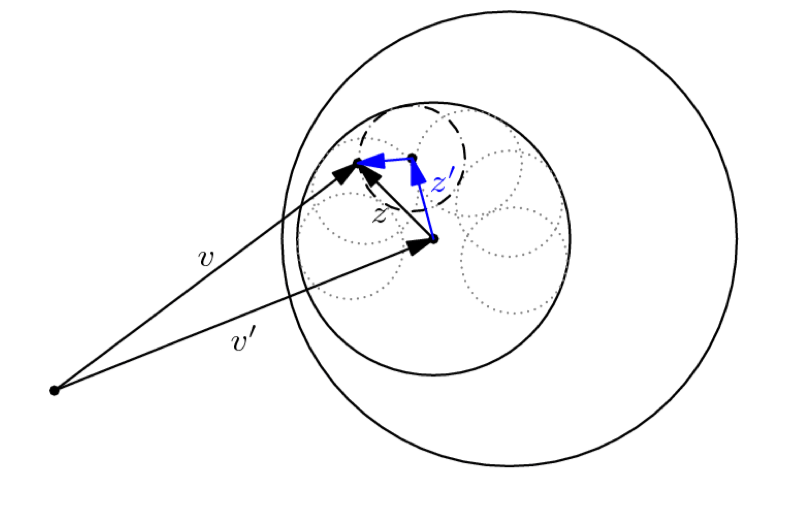
\includegraphics[width=0.7\textwidth]{Figs/4.png}
    \caption{Illustration of a chained cover. Within the $\epsilon$-ball containing the discretization error $z$, we find a finer $\epsilon^{\prime}$-cover and obtain a smaller error $z^{\prime}$ from discretizing $z$.}
    \label{fig:chain}
\end{figure}
It is possible to obtain a stronger theorem by constructing a \tb{chained $\epsilon$-covering scheme.} Specifically, when we decompose $v=v^{\prime}+z$, we can construct a finer-grained covering of the ball $B\left(v^{\prime}, \epsilon\right)$, and then we can decompose $z$ into smaller components and so on (see \cref{fig:chain}). 

\tb{\centerline{Chaining is not an uniformly sized cover.}}

Using this method of chaining, we can obtain the following (stronger) result:
\begin{thma}\bfs{Dudley's Theorem}\label{thm:Dudley's Theorem}
 If $\mathcal{F}$ is a function class from $Z$ to $\mathbb{R}$, then
\begin{align}
R_{S}(\mathcal{F}) \leq 12 \int_{0}^{\infty} \sqrt{\frac{\log N\left(\epsilon, \mathcal{F}, L_{2}\left(P_{n}\right)\right)}{n}} d \epsilon\label{eq:hqcfdf}
\end{align}
\end{thma}
\begin{rema}
We can interpret this bound as removing the discretization error term of \cref{thm:frtyzc} by \tb{averaging over different scales of $\epsilon$}. For a proof of this theorem, refer to Theorem 15 of \cite{Liang}.
If $\mathcal{F}$ consists of functions bounded in $[-1,1]$, then, we have that for all $\epsilon>1, N\left(\epsilon, \mathcal{F}, L_{2}\left(P_{n}\right)\right)=1$. (To see this choose $\{f \equiv 0\}$, which is a complete cover for $\epsilon>1 .)$ Hence, the limits of integration in \cref{eq:hqcfdf} can be truncated to $[0,1]$ :
\begin{align*}
R_{S}(\mathcal{F}) \leq 12 \int_{0}^{1} \sqrt{\frac{\log N\left(\epsilon, \mathcal{F}, L_{2}\left(P_{n}\right)\right)}{n}} d \epsilon
\end{align*}
since $\log N\left(\epsilon, \mathcal{F}, L_{2}\left(P_{n}\right)\right)=0$ for $\epsilon>1$.
\end{rema}
\subsubsection{Covering Number Regimes for Which Dudley's Theorem is Finite}
Of course, the bound in \cref{eq:hqcfdf} is only useful if the integral on the RHS is finite. Here are some setups where this is the case (we continue to assume that the functions in $\mathcal{F}$ are bounded in $[-1,1]$):
\begin{enumerate}
    \item If $N\left(\epsilon, \mathcal{F}, L_{2}\left(P_{n}\right)\right) \approx(1 / \epsilon)^{R}$ (ignoring multiplicative and additive constants), then we have $\log N\left(\epsilon, \mathcal{F}, L_{2}\left(P_{n}\right)\right) \approx R \log (1 / \epsilon)$. We can plug this into the RHS of \cref{eq:hqcfdf} ) to get
\begin{align*}
\int_{0}^{1} \sqrt{\frac{\log N\left(\epsilon, \mathcal{F}, L_{2}\left(P_{n}\right)\right)}{n}} d \epsilon=\int_{0}^{1} \sqrt{\frac{R \log (1 / \epsilon)}{n}} d \epsilon \approx \sqrt{\frac{R}{n}}
\end{align*}
\item If the covering number has the form $N\left(\epsilon, \mathcal{F}, L_{2}\left(P_{n}\right)\right) \approx a^{R / \epsilon}$ for some $a$, then we have $\log N\left(\epsilon, \mathcal{F}, L_{2}\left(P_{n}\right)\right) \approx \frac{R}{\epsilon} \log a$. The bound in \cref{eq:hqcfdf} becomes
\begin{align*}
\begin{aligned}
\int_{0}^{1} \sqrt{\frac{\log N\left(\epsilon, \mathcal{F}, L_{2}\left(P_{n}\right)\right)}{n}} d \epsilon & \approx \int_{0}^{1} \sqrt{\frac{R}{n \epsilon} \log a} d \epsilon \\
&=\sqrt{\frac{R}{n} \log a} \int_{0}^{1} \sqrt{\frac{1}{\epsilon}} d \epsilon \\
&=\widetilde{O}\left(\sqrt{\frac{R}{n}}\right)
\end{aligned}
\end{align*}
\item If the covering number has the form $N\left(\epsilon, \mathcal{F}, L_{2}\left(P_{n}\right)\right) \approx a^{R / \epsilon^{2}}$, then $\log N\left(\epsilon, \mathcal{F}, L_{2}\left(P_{n}\right)\right) \approx \frac{R}{\epsilon^{2}} \log a$. In this case we have:
\begin{align*}
\int_{0}^{1} \sqrt{\frac{\log N\left(\epsilon, \mathcal{F}, L_{2}\left(P_{n}\right)\right)}{n}} d \epsilon \approx \sqrt{\frac{R}{n} \log a} \underbrace{\int_{0}^{1} \frac{1}{\epsilon} d \epsilon}_{=\infty}=\infty
\end{align*}
i.e. the bound in \cref{eq:hqcfdf} is vacuous. This is because of the behavior of $\epsilon \mapsto 1 / \epsilon^{2}$ near 0: the function goes to infinity too quickly for us to upper bound its integral. Fortunately, there is an "improved" version of Dudley's theorem that is applicable here:
\end{enumerate}
\begin{thma}\bfs{Improved Dudley's Theorem}
 If $\mathcal{F}$ is a function class from $Z$ to $\mathbb{R}$, then for any fixed cutoff $\alpha \geq 0$ we have the bound
\begin{align*}
R_{S}(\mathcal{F}) \leq 4 \alpha+12 \int_{\alpha}^{\infty} \sqrt{\frac{\log N\left(\epsilon, \mathcal{F}, L_{2}\left(P_{n}\right)\right)}{n}} d \epsilon
\end{align*}
\end{thma} 
\begin{rema}
The proof of this theorem is similar to the proof of the original Dudley's theorem, except that the iterative covering procedure is stopped at the threshold $\epsilon=\alpha$ at the cost of the extra $4 \alpha$ term above. Theorem $4.28$ allows us to avoid the problematic region around $\epsilon=0$ in the integral in \cref{eq:hqcfdf}. If we let $\alpha=1 /$ poly $(n)$, the bound in $(4.117)$ becomes
\begin{align*}
\begin{aligned}
R_{S}(\mathcal{F}) & \leq \frac{1}{p o l y(n)}+\frac{\sqrt{R \log a}}{\sqrt{n}} \int_{\alpha}^{1} \frac{1}{\epsilon} d \epsilon \\
&=\frac{1}{p o l y(n)}+\frac{\sqrt{R \log a}}{\sqrt{n}} \log (1 / \alpha) \\
&=\widetilde{O}\left(\sqrt{\frac{R}{n}}\right)
\end{aligned}
\end{align*}
\end{rema}

$\bullet$ \tb{Summary:}  
\begin{enumerate}
    \item We have that $R_{S}(\mathcal{F}) \leq \widetilde{O}\left(\sqrt{\frac{R}{n}}\right)$ for these three dependencies on $\epsilon:$ when $\log N\left(\epsilon, \mathcal{F}, L_{2}\left(P_{n}\right)\right) \approx R \log (1 / \epsilon), \frac{R}{\epsilon} \log a$, or $\frac{R}{\epsilon^{2}} \log a$ for some $a$.
    \item Note that if the dependence on $\epsilon$ is $1 / \epsilon^{c}$ for $c>2$, then even the improved Dudley's theorem does not help us. This is because the log $(1 / \alpha)$ term above becomes $\alpha^{1-c / 2}$, and when $\alpha=1 / \operatorname{poly}(n)$, this term leads to a bad dependence on $n$
\end{enumerate}
\subsubsection{Special Situations where We Can Get Covering Number Bounds}
The previous remarks discuss how strong our bounds on covering number need to be in order to get a useful result. Here we mention some situations in which we know how to obtain these covering number bounds:
\begin{enumerate}
    \item Covering number and corresponding Rademacher complexity bounds for \tb{linear models} are well-known, but fairly technical (see \cite{zhang2002covering}).
    \item \tb{Covering numbers interact nicely with composition by Lipschitz functions.} If $\phi$ is a $\rho$-Lipschitz function, then the following bound holds:
\begin{align*}
N\left(\epsilon / \rho, \mathcal{F}, L_{2}\left(P_{n}\right)\right) \geq N\left(\epsilon, \phi \circ \mathcal{F}, L_{2}\left(P_{n}\right)\right)
\end{align*}
This result is the analog of Talagrand's lemma for covering numbers. The proof follows easily if one considers $\phi$ as a change of measure: informally, the Lipschitz condition on $\phi$ means that a distance of $\epsilon / \rho$ in the original space $\mathcal{F}$ can be increased to at most $\epsilon$ in the space $\phi \circ \mathcal{F}$.
\item Using these results we can obtain a bound on the Rademacher complexity of a \tb{dense neural network}. Consider a deep network
\begin{align*}
f(x)=W_{r} \sigma\left(W_{r-1} \sigma\left(\cdots \sigma\left(W_{1} x\right) \ldots\right)\right.
\end{align*}
where $W_{i}$ are layer-wise weights and $\sigma$ is an activation function which is $1$-Lipschitz. For this setup we have the following Rademacher complexity bound:
\begin{align*}
R_{S}(\mathcal{F}) \leq \underbrace{\left(\prod_{i=1}^{r}\left\|W_{i}\right\|_{\mathrm{op}}\right)}_{\text {relatively large }} \cdot \underbrace{\left(\sum_{i=1}^{r} \frac{\left\|W_{i}^{T}\right\|_{2,1}^{2 / 3}}{\left\|W_{i}\right\|_{\mathrm{op}}^{2 / 3}}\right)^{3 / 2}}_{\text {relatively small }}
\end{align*}
Here $\|W\|_{\text {op }}$ is the operator norm (or spectral norm) of $W$, and $\left\|W_{i}^{T}\right\|_{2,1}$ denotes the sum of the $l_{2}$ norms of the rows of $W_{i} .$ The second term is relatively small as it is a sum of matrix norms, and so the bound is dominated by the first term, which is a product of matrix norms. This first term comes from composition of Lipschitz functions as above, since the \tb{Lipschitz constant of a linear operator is its spectral norm.} The full details are presented in \cite{bartlett2017spectrally}.
\end{enumerate}
\subsection{VC Dimension and Its Limitations}
We will focus on classification and will be working within the framework of supervised learning stated in Chapter 1. The labels belong to the output space $\mathcal{Y}=\{-1,1\}$, each classifier is a function $h: \mathcal{X} \rightarrow \mathbb{R}$ for all $h \in \mathcal{H}$, and the prediction is the sign of the output, i.e. $\hat{y}=\operatorname{sgn}(h(x)) .$ We will look at zero-one loss, i.e. $\ell_{0-1}((x, y), h)=\mathbb{1}(\operatorname{sgn}(h(x)) \neq y) .$ Note that we can re-express the loss function as
\begin{align*}
\ell_{0-1}((x, y), h)=\frac{1-\operatorname{sgn}(h(x)) y}{2}
\end{align*}
The first approach is to reason directly about the Rademacher complexity of $\ell_{0-1}$ loss, i.e. considering the family of functions $\mathcal{F}=\left\{z=(x, y) \mapsto \ell_{0-1}((x, y), h): h \in \mathcal{H}\right\} .$ Define $Q$ to be the set of all possible outputs

on our dataset: $Q=\left\{\left(\operatorname{sgn}\left(h\left(x^{(1)}\right)\right), \ldots, \operatorname{sgn}\left(h\left(x^{(n)}\right)\right)\right) \mid h \in \mathcal{H}\right\} .$ Then, using our earlier remark about viewing the empirical Rademacher complexity as an inner product between $v \in Q$ and $\sigma$, we have
\begin{align*}
\begin{aligned}
R_{S}(\mathcal{F}) &=\mathbb{E}_{\sigma_{1}, \ldots, \sigma_{n}}\left[\sup _{f \in \mathcal{F}} \frac{1}{n} \sum_{i=1}^{n} \sigma_{i} \frac{1-\operatorname{sgn}\left(h\left(x^{(i)}\right)\right) y_{i}}{2}\right] \\
&=\mathbb{E}_{\sigma_{1}, \ldots, \sigma_{n}}\left[\sup _{f \in \mathcal{F}} \frac{1}{n} \sum_{i=1}^{n} \sigma_{i} \frac{\operatorname{sgn}\left(h\left(x^{(i)}\right)\right)}{2}\right] \\
&=\frac{1}{2} \mathbb{E}_{\sigma_{1}, \ldots, \sigma_{n}}\left[\sup _{v \in Q} \frac{1}{n}\langle\sigma, v\rangle\right]
\end{aligned}
\end{align*}
Notice that the supremum is now over $Q$ instead of $\mathcal{F} .$ If $n$ is sufficiently large, then it is typically the case that $|Q|>|\mathcal{F}| .$ To see why this is the case, note that each function $f$ corresponds to a single element in $Q .$ However, as $n$ increases, $|Q|$ increases as well. For any particular $v \in Q$, notice that $\langle v, \sigma\rangle$ is a sum of bounded random variables, so we can use Hoeffding's inequality to obtain
\begin{align*}
\operatorname{Pr}\left[\frac{1}{n}(\sigma, v) \geq t\right] \leq \exp \left(-n t^{2} / 2\right)
\end{align*}
Taking the union bound over $v \in Q$, we see that
\begin{align*}
\operatorname{Pr}\left[\exists v \in Q \text { such that } \frac{1}{n}\langle\sigma, v\rangle \geq t\right] \leq|Q| \exp \left(-n t^{2} / 2\right)
\end{align*}
Thus, with probability at least $1-\delta$, it is true that $\sup _{v \in Q} \frac{1}{n}\langle v, \sigma\rangle \leq \sqrt{\frac{2(\log |Q|+\log (2 / \delta))}{n}}$. Similarly, we can show that $\mathbb{E}\left[\sup _{v \in Q} \frac{1}{n}\langle v, \sigma\rangle\right] \leq O\left(\sqrt{\frac{\log |Q|+\log (2 / \delta)}{n}}\right)$ holds.

The key point to notice here is that the upper bound on $R_{S}(\mathcal{F})$ depends on $\log |Q| . V C$ dimension is one way that we deal with bounding the size of $Q$ We will not delve into the details of this approach (for those interested, see Section $3.11$ of $[\mathrm{Liang}, 2016 \mid) .$ VC dimension, however, has a number of limitations. For one, we will always end up with a bound that depends somehow on the dimension. For linear models, we obtain a bound $\log |Q| \lesssim d \log n$, corresponding to a bound on Rademacher complexity that looks like
\begin{align*}
R_{S}(\mathcal{F}) \leq \widetilde{O}\left(\sqrt{\frac{d}{n}}\right)
\end{align*}
so we still have a $\sqrt{d}$ term. This will not be a good bound for high-dimensional models. For general models, we will arrive a bound of the form
\begin{align*}
R_{S}(\mathcal{F}) \leq \widetilde{O}\left(\sqrt{\frac{\# \text { of parameters }}{n}}\right)
\end{align*}
This upper bound only depends on the number of parameters in our model, and does not take into the account the scale and norm of the parameters. Additionally, this doesn't work with kernel methods since the explicit parameterization is possibly infinite-dimensional, and therefore this upper bound becomes useless.
These limitations motivation the use of margin theory, which does take into account the norm of parameters and provides a theoretical basis for regularization techniques such as $L_{1}$ and $L_{2}$ regularization.

\section{Rademacher Complexity Bounds for Concrete Models and Losses}\label{sec:radcom_conc}
\bibliographystyle{IEEEtran}
\bibliography{IEEEabrv,StringDefinitions,adv_dnn}
\end{document}